\documentclass[conference]{IEEEtran}
\usepackage[hidelinks,hypertexnames=false]{hyperref}
\usepackage{graphicx}
\usepackage{cite}
\usepackage{float}
\usepackage{enumitem}
\usepackage{booktabs}
\usepackage{array}
\usepackage{url}
\usepackage{amsmath}
\usepackage{xcolor}
\usepackage{tikz}
\usetikzlibrary{arrows.meta,positioning}

\title{SimpleChef: Progress Report\\Human Computer Interaction (CS4063)}
\author{%
\IEEEauthorblockN{Drew Skelton, Trinity Tran, Colby Frison, Carson Petty, Reese Booker }
\IEEEauthorblockA{SimpleChef - Spring 2026 \\ March 29, 2026}}

\setlength{\defaultaddspace}{3pt}

\begin{document}
\graphicspath{{figures/}}
\maketitle

\begin{abstract}
This progress report summarizes development of SimpleChef, a mobile-first cooking assistant built with React Native (Expo), FastAPI, and PostgreSQL. We describe objectives aligned with our project proposal, \textbf{implemented features as of March~29,~2026}, including a \textbf{controller-based frontend architecture} that separates application logic from presentation for easy implementation of Figma UI designs. Towards the end of this report we shows evidence of implementation through high-fidelity UI designs (Section~\ref{sec:evidence}), these screens are not yet connected to the live API in the repository, but the backend endpoints are already established for each flow, and connection is planned through the existing controller hooks. We summarize ongoing gaps in implementation, remaining work, project workflow/architecture figures, and an updated milestone timeline toward final delivery.
\end{abstract}

\section{Project Overview}
SimpleChef is a mobile-first cooking assistant designed to reduce friction across the entire cooking process - from discovering a recipe to meal planning and grocery shopping. The tagline \emph{Your calm kitchen companion} reflects the goal of a capable, calm tool that streamlines everyday cooking tasks.

As stated in our project proposal, many cooking apps fragment the experience: recipes in one place, calories in another, and a grocery lists on paper or in notes that has to be meticulously organized. Instructions often appear as long blocks of text, and timers frequently push users out of the recipe context. SimpleChef targets a single cohesive flow: recipe discovery, step-by-step cooking with integrated timers, meal planning with calorie awareness, and grocery support. The design applies HCI ideas including progressive disclosure, clarity over clutter, and smart defaults with full user control~\cite{preece2015,hartson2012ux}.

\subsection{Objectives}
\begin{itemize}[leftmargin=*]
  \item \textbf{Unify the workflow} across browsing, cooking mode, planning, and groceries with consistent navigation and data flow.
  \item \textbf{Optimize step-by-step cooking} so each step is scannable during active cooking, with integrated timers and ingredients tied to steps where modeled.
  \item \textbf{Timer management} via a timer dock that surfaces active timers without leaving the cooking context.
  \item \textbf{Grocery automation} from planned meals (deduplication, categories, merge from plan, export).
  \item \textbf{Lower recipe input friction} via manual entry plus AI-assisted text parsing* with verification before save, image and video import remain planned.
  \item \textbf{Meal planning and calorie goals} by assigning meals to days, day-level calorie summaries vs.\ profile goals, and recipe filters (API); richer statistics (macronutrients) are planned to be added by allowing extensions.
  \item \textbf{Iterate with users} through feedback sessions and refinement of flows and visuals~\cite{nielsen1994heuristic}.
\end{itemize}

\subsection{Tools and technology}
\begin{itemize}[leftmargin=*]
  \item \textbf{Frontend:} React Native (Expo). Routes under through front ends, and \textbf{application logic} is centralized in the controller pattern (hooks such as \texttt{useRecipeLibraryController}, \texttt{usePlannerController}, \texttt{useGroceryController}) so screens stay presentation-focused and can be mirrored in Figma without duplicating API rules. Shared DTOs live in the front end as well, and HTTP and auth live in the services directory
  \item \textbf{Backend:} FastAPI (Python) with SQLAlchemy models and Alembic migrations; JWT auth for protected routes.
  \item \textbf{Data store:} PostgreSQL (via Docker Compose for local development).
  \item \textbf{Design:} Figma for wireframes and high-fidelity exploration~\cite{figma2026help}; repository documentation (Section~\ref{sec:repo-docs}) lists every named UI/API requirement for annotation without duplicating them in this PDF.
  \item \textbf{AI/ML:} Text parsing uses a structured placeholder/demo path with validation. Production LLM/vision is not part of the requirements for our current milestone.
\end{itemize}

\section{Repository documentation}
\label{sec:repo-docs}
We have extremely detailed system requirements and specification in our shared repository, so we easily and reliably recall what still needs to implemented, what is currently implemented, and the specifications of all features. This also makes UI and system design easy as we have all needed elements already laid out. We have these documents in our /docs directory of our shared repository. But the repository is private so we will be unable to share it, if you would like to see the repository we would be happy to let you view it in class, or through office hours if time permits.

\newpage

\section{Project Progress Overview}
As of March~29,~2026, the team has parts of the system functional: an Expo client showing a model frontend (which is ready for the high-fidelity veriosn), FastAPI APIs of the backend, and a functional PostgreSQL database that supports authentication and interacts with essentially all of the main tabs and core flows described in the proposal. The frontend follows a controller patter layer that has route files that bind UI pages to hooks that encapsulate loading state, validation, and service calls. This permits a full sepeartion between layers, mitigating large ssytem wide errors.

\subsection{Completed milestones and components}
\begin{itemize}[leftmargin=*]
  \item \textbf{Proposal and design specification:} Scope, problem statement, five-tab UI navigation system (Home, Calendar, Add, Grocery, Profile), wireframe, and timeline documented.
  \item \textbf{Backend foundation:} Application entry points, models for users (database integration), recipes (ingredients, steps), meal plans, grocery lists/items, and versioned migrations.
  \item \textbf{Authentication:} Signup and login for authentication, JWT via Axios interceptor,  recipe visibility and ownership enforced server-side via database permissions.
  \item \textbf{Recipe library:} Debounced search, difficulty chips, RecipeList fed by \texttt{useRecipeLibraryController}; API supports additional filters (\texttt{max\_total\_minutes}, \texttt{tags\_all}) for future UI.
  \item \textbf{Recipe detail:} Hero image or placeholder, summary stats, expandable ingredients, steps; Begin Cooking; add to calendar modal; owner edit/delete.
  \item \textbf{Cooking mode:} Step navigation, progress, prep/ingredients per step (ingredient - step linking), timer dock (\texttt{TimerDock}, \texttt{useTimerStore}), optional per-step timers, ``all ingredients'' modal, keep-awake when profile requests it.
  \item \textbf{Add recipe:} Manual form with dynamic rows; paste flow calls \texttt{POST /recipes/parse} and opens verification on the manual screen. Image scan remains disabled (\emph{Coming Soon}).
  \item \textbf{Meal planner:} Month grid, selected day, meals list, quick add, add from recipe library with meal type, delete; \texttt{GET /planner/day-summary} supports consumed calories vs.\ profile goal on the calendar screen.
  \item \textbf{Grocery list:} Sectioned list, checkbox sync, manual add, merge from meal plan (date range), share/export text.
  \item \textbf{Profile:} Edit name, bio, calorie goal, dietary restrictions (comma-separated), keep-screen-on toggle; save via \texttt{PATCH /users/me}; friends/social is out of scope for this build, but hopefully we can get a simple version of it implemented to find recipes to make building a recipe library easier.
\end{itemize}

\subsection{Gaps relative to the proposed UI and SRS (Software Requirement Specification)} 
\begin{itemize}[leftmargin=*]
  \item \textbf{Home:} Filter drawer (cook time, profile-default dietary tags) not fully exposed in UI though API supports several query parameters.
  \item \textbf{Cooking mode:} proposal describe replacing the bottom tab bar with cooking-specific chrome; current app keeps stack navigation inside the tab shell - this may remain as it acts as an easy exit point out of the page, user testing may change this outlook however.
  \item \textbf{Calendar:} Color coding by meal type, and statistics charts are not implemented. Out of all parts of the application the calendar likely needs the most refinement - it is difficult as having all days listed while not feeling cluttered is difficult, especially on a mobile device.
  \item \textbf{Grocery:} Full inline editor and drag-to-reorder categories are not implemented; merge and check-off work.
  \item \textbf{AI parsing:} Demo/placeholder parser, not a production LLM or vision pipeline.
  \item \textbf{Friends / social:} Out of scope per backlog; proposal text remains for future product direction.
\end{itemize}

\section{Ongoing Challenges and Design Difficulties}
\subsection{Closing the loop among meal plans, recipes, and groceries}
The proposal promises a grocery list grounded in planned meals. A merge path aggregates ingredients from planned recipes in a date range; users can still edit items manually. Modifying recipes to work per serving will require some logic adjustment and research on ratios in cooking.

\subsection{Search, filter, and dietary personalization}
Server-side filters exist; the Home UI should expose time caps and tag filters aligned with profile dietary strings to limit choice overload on Home~\cite{hartson2012ux}.

\subsection{In place instructions and step granularity}
Ingredients can link to steps; the cooking screen shows global prep on step one and step-linked items thereafter. Parsing quality and editor UX for linking remain improvement areas.

\subsection{Trustworthy AI parsing}
A mock parser can mislead participants about accuracy. A real text parser behind the same verify-and-edit screen, with image/video clearly labeled beta, although not a high priority task it is still important~\cite{nielsen1994heuristic}.

\subsection{Calendar information density}
Month grid exists; richer at-a-glance indicators and proposal-style bottom sheet are partial. Usability tests should compare taps-to-complete for ``add from library.''

\subsection{Engineering and maintainability}
Cross-cutting concerns (authorization, validation boundaries, service vs.\ router responsibilities) are recorded in the project for future refactors without blocking feature delivery to retain project stability.

\section{Implementation Evidence}
\label{sec:evidence}

The following figures are \textbf{high-fidelity UI designs} (phone aspect ratio) captured for this report. They are organized by feature area (e.g. profile, login, home, etc.). These designs are not yet connected to the running backend in the main repo as there is still some refinement to be done, but the backend is set up with specific exposed APIs so it is very easy to connect and modify the frontend. \textbf{For every screen shown below, a corresponding backend already exists} in the repository (e.g., auth, recipes, planner, etc.) which is all documented in our shared repository. Because of this no new architectural pattern is required, all we have to so is write each view to the appropriate controller and DTO types, which is much more simple than having to rewrite large connections.

\subsection{Frontend Implementation}

\textbf{Authentication (sign-in and registration) - } This page has two main sections, one for returning users and the other for new users. Users will remain logged in when the app is closed, but when they are using a new device they will have to log in still, hence why a login screen is present. For new users there is a page to create an account, which only requires the simple info typical of a login screen. In the future, we may add a next step to this new user account creation that will consist of a walkthrough of the app's functions and a prompt to enter other account details (e.g. goals, dietary restrictions, etc.), making this lead into onboarding rather than just throwing new users into the app.

\begin{figure}[!htbp]
\centering
\begin{minipage}[!htbp]{0.46\linewidth}\centering
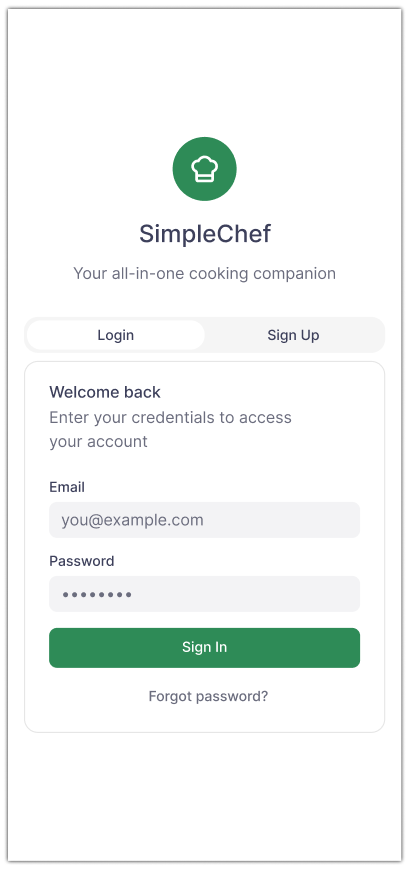
\includegraphics[width=\linewidth]{auth/login.png}\\[0.15em]
\scriptsize Login
\end{minipage}
\begin{minipage}[!htbp]{0.46\linewidth}\centering
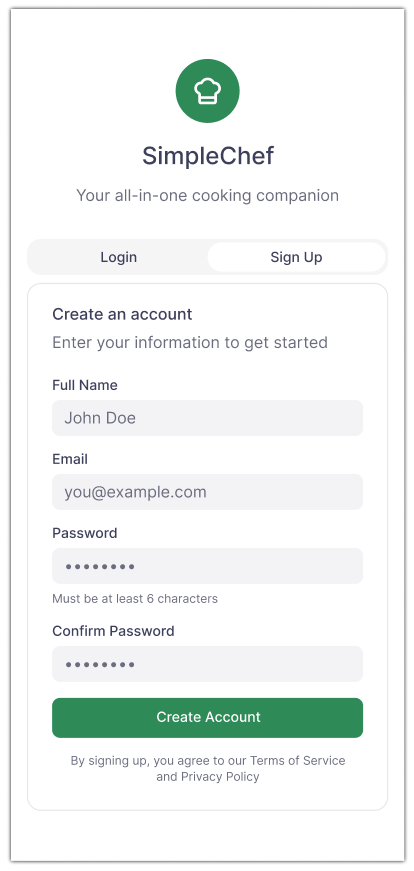
\includegraphics[width=\linewidth]{auth/create-account.png}\\[0.15em]
\scriptsize Create account
\end{minipage}
\caption{Authentication: email/password login and account creation. }
\label{fig:auth}
\end{figure}

\newpage
\textbf{Home (recipe library) - }This page is the home screen which consists of a list of recipes viewable by scrolling, this list can be filtered by a variety of tags which can be applied to recipes for easier searching. These tags are a stand in for now, but in later implementations they will likely be based on tags already one existing food so there is no redundancy.

\begin{figure}[!htbp]
\centering
\begin{minipage}[!htbp]{0.35\linewidth}\centering
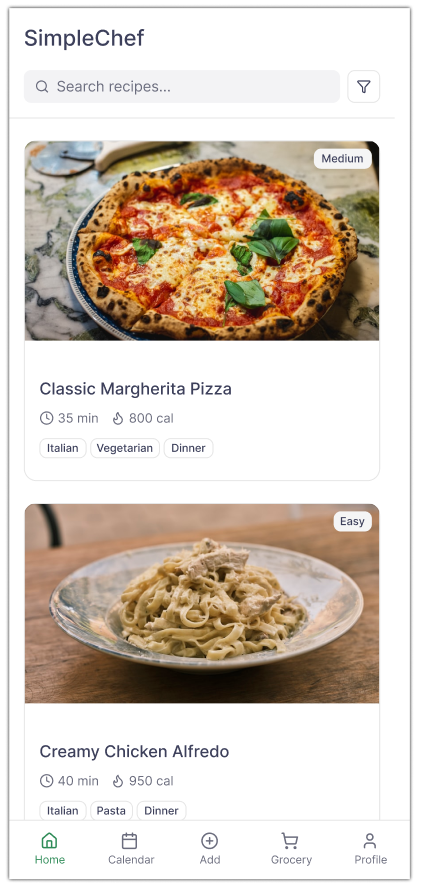
\includegraphics[width=\linewidth]{home/home.png}\\[0.15em]
\scriptsize Home (library)
\end{minipage}
\begin{minipage}[!htbp]{0.35\linewidth}\centering
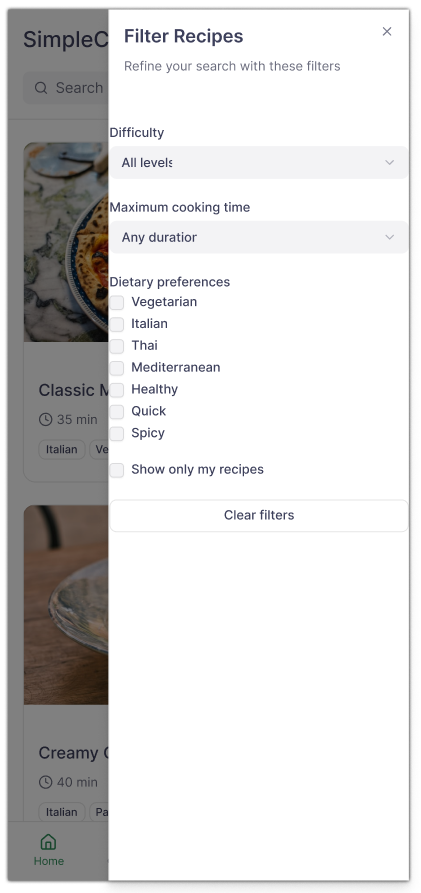
\includegraphics[width=\linewidth]{home/home-filter.png}\\[0.15em]
\scriptsize Search and filter chips
\end{minipage}
\caption{Home screen: List of recipes and filter menu.}
\label{fig:home}
\end{figure}

\textbf{Recipe detail - } The following is what a user sees when a recipe is clicked, it contains a short overview of the recipe along with everything the user would need before starting the recipe. The user can also edit and remove this recipe from this submenu with the icons in the top right, and go back to the home screen with the arrow in the top left. The edit menu is the same as the recipe creation menu which will be seen shortly.

\begin{figure}[!htbp]
\centering
\begin{minipage}[!htbp]{0.35\linewidth}\centering
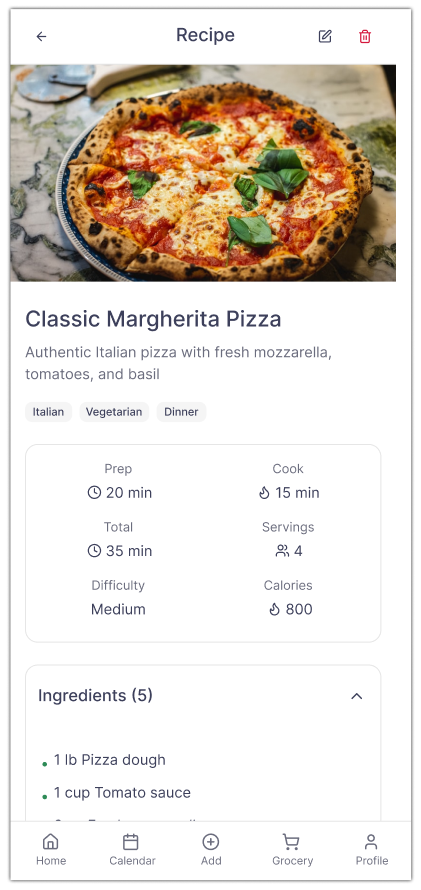
\includegraphics[width=\linewidth]{home/recipe-top.png}\\[0.15em]
\scriptsize Recipe detail (top)
\end{minipage}
\begin{minipage}[!htbp]{0.35\linewidth}\centering
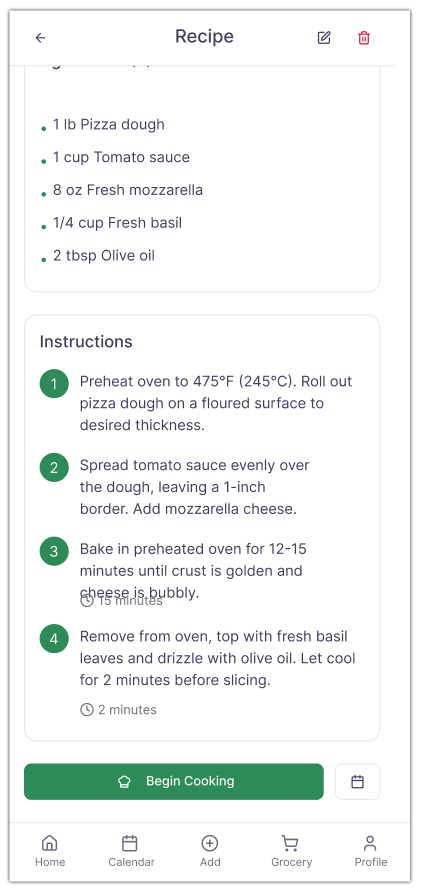
\includegraphics[width=\linewidth]{home/recipe-bottom.png}\\[0.15em]
\scriptsize Recipe detail (bottom)
\end{minipage}
\caption{Recipe detail (scroll): summary, ingredients, and actions. Controller: \texttt{useRecipeDetailController}. API: \texttt{GET /recipes/\{id\}}.}
\label{fig:recipe-detail}
\end{figure}

\newpage
\textbf{Help / instructions - } The following is still very much a work in progress, but it is the guided recipe screen a user will see when a recipe is started. There are buttons at the bottom to see progress and go forward or back, along with an indicator of progress. The timer button is visible in the instructions and when started appears at the bottom, which can be used to pause or cancel the timer. The button in the top right can be selected to see all the ingredients for the recipe. This is one of many iterations of these menus, and there are likely going to be a few more until we land on a final product.

\begin{figure}[!htbp]
\centering
\begin{minipage}[!htbp]{0.35\linewidth}\centering
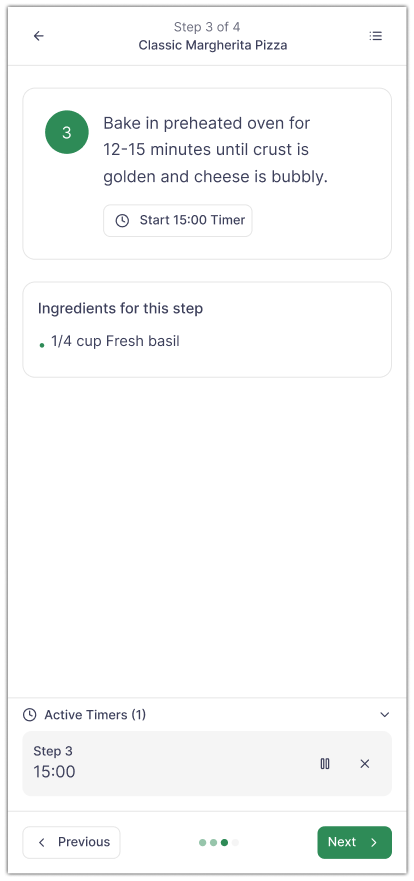
\includegraphics[width=\linewidth]{home/instructions.png}\\[0.15em]
\scriptsize Instructions (full screen)
\end{minipage}
\begin{minipage}[!htbp]{0.35\linewidth}\centering
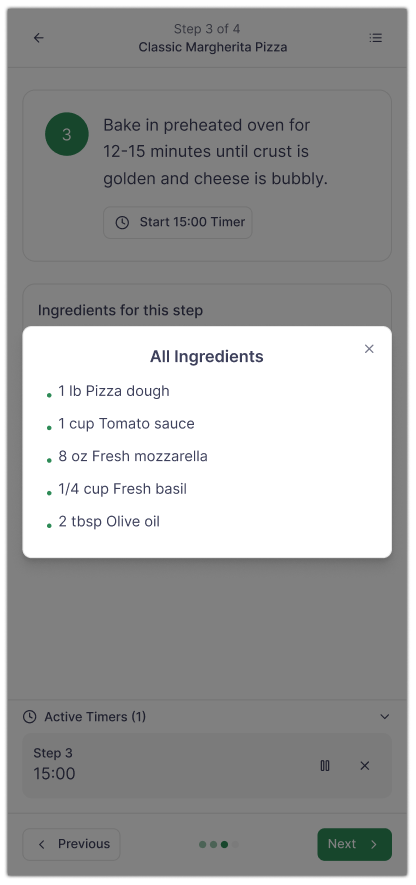
\includegraphics[width=\linewidth]{home/instructions-modal.png}\\[0.15em]
\scriptsize Instructions (modal)
\end{minipage}
\caption{Onboarding or help for library search and filters (draft labels). Not tied to a single API route; supports discoverability on Home.}
\label{fig:filters-help}
\end{figure}

\textbf{Calender - } This page contains the calendar for the month, and is the main way to plan recipes/meals for the user. Days can be selected by clicking on them, and the current day is selected by default. When meals are added to a day they are shown via dots on the selected day, and when the day is selected the meals and calories are shown.

\begin{figure}[!htbp]
\centering
\begin{minipage}[!htbp]{0.35\linewidth}\centering
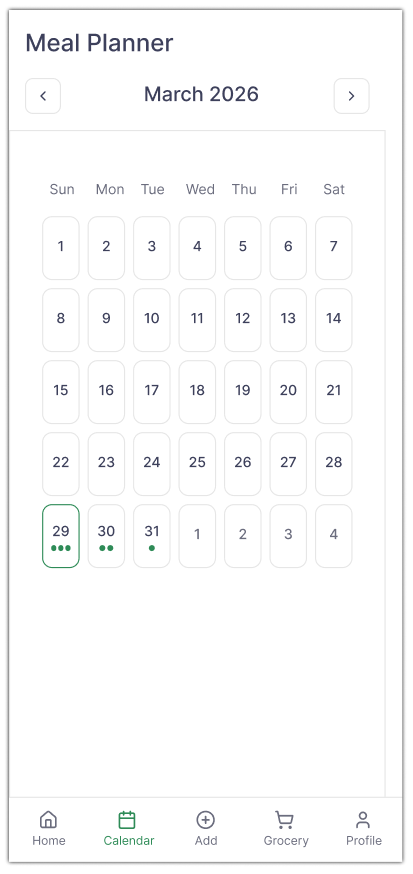
\includegraphics[width=\linewidth]{calendar/calendar.png}\\[0.15em]
\scriptsize Month grid
\end{minipage}
\begin{minipage}[!htbp]{0.35\linewidth}\centering
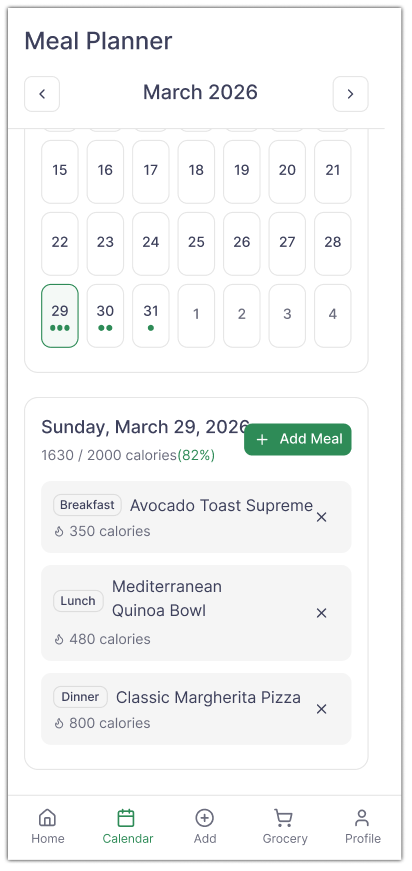
\includegraphics[width=\linewidth]{calendar/calendar-day-selected.png}\\[0.15em]
\scriptsize Day selected
\end{minipage}
\caption{Calendar: month overview and highlighted date.}
\label{fig:calendar-month}
\end{figure}

\newpage
\textbf{Empty day/Adding meal - } The first image is what appears when a day with nothing planned is selected, prompting the user to select a meal. The second image is the modal that appears when the add meal button is selected providing the options to select a recipe from the user library, or to input a custom food (e.g. a snack, or a purchased meal).

\begin{figure}[!htbp]
\centering
\begin{minipage}[!htbp]{0.39\linewidth}\centering
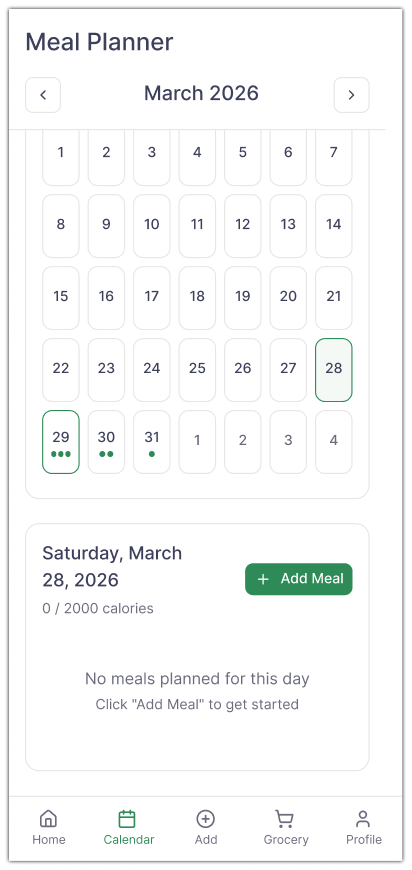
\includegraphics[width=\linewidth]{calendar/calendar-empty.png}\\[0.15em]
\scriptsize Empty day
\end{minipage}
\begin{minipage}[!htbp]{0.39\linewidth}\centering
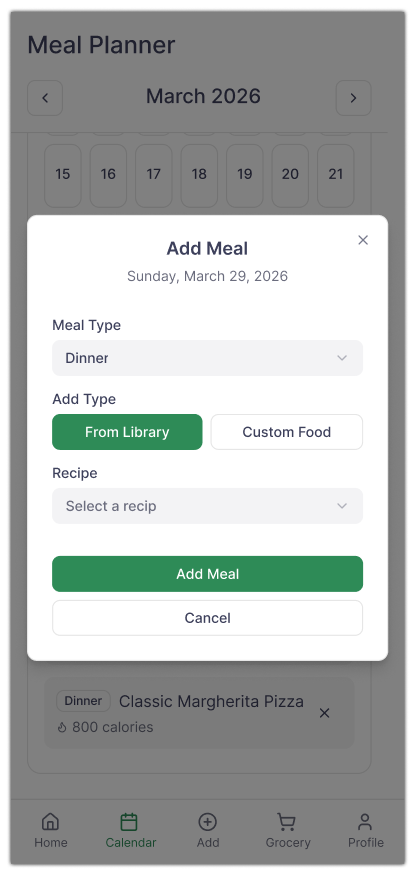
\includegraphics[width=\linewidth]{calendar/calender-add-modal.png}\\[0.15em]
\scriptsize Add meal (planner modal)
\end{minipage}
\caption{Planner: empty day and add-meal dialog. }
\label{fig:planner-day}
\end{figure}

\textbf{Add recipe - } This is where a user will input a recipe, right now there are only two options, but hopefully in the future we can add more options to input recipes. The main and only functional method right now is manually entering the recipe which is done with the latter 2 images. The first image is the soon-to-be implemented AI parsing of a recipe which will (hopefully) use AI/ML to parse input text into a recipe that can then be edited and saved.

\begin{figure}[!htbp]
\centering
\begin{minipage}[!htbp]{0.31\linewidth}\centering
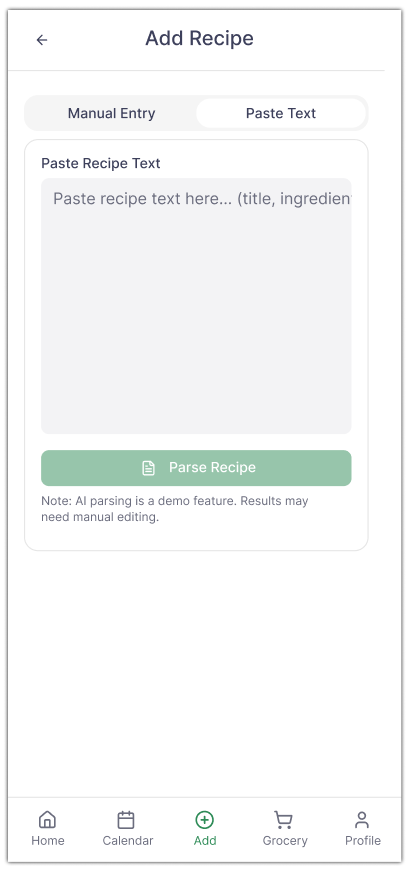
\includegraphics[width=\linewidth]{add/ai.png}\\[0.15em]
\scriptsize Add recipe (paste / AI)
\end{minipage}\hfill
\begin{minipage}[!htbp]{0.31\linewidth}\centering
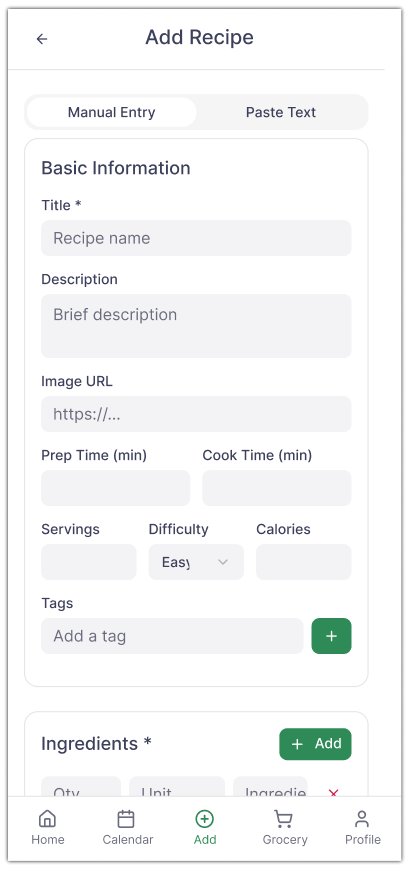
\includegraphics[width=\linewidth]{add/manual-bottom.png}\\[0.15em]
\scriptsize Manual entry (bottom)
\end{minipage}\hfill
\begin{minipage}[!htbp]{0.31\linewidth}\centering
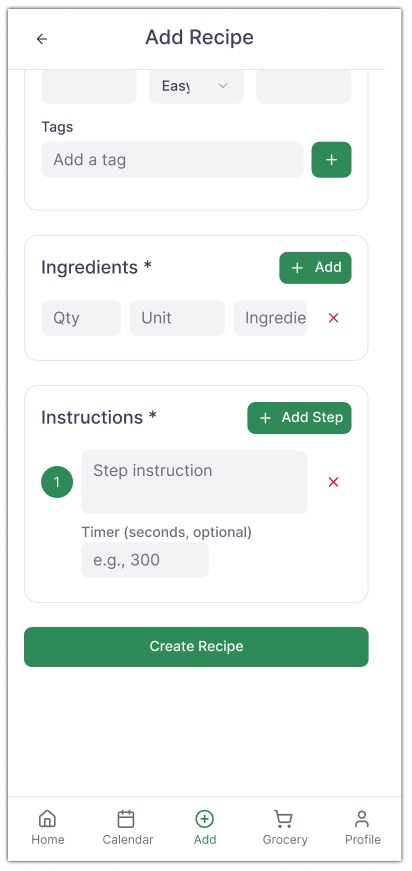
\includegraphics[width=\linewidth]{add/manual-top.png}\\[0.15em]
\scriptsize Manual entry (top)
\end{minipage}
\caption{Add recipe: import entry point and manual create/edit form.}
\label{fig:add-recipe}
\end{figure}

\newpage
\textbf{Grocery list - } This page contains a checklist of ingredients/items for a shopping list that can be autogenerated based on the meals planned for the following week, or items can be added manually. Added items can be checked off or removed from the interface, and they can also be exported, which right now just copies the list to the clipboard so it can be pasted in another app presumably the notes app, but in the future we hope to figure out how to connect it to service like the Instacart or the Walmart app, so groceries can be easily be ordered instead.

\begin{figure}[!htbp]
\centering
\begin{minipage}[!htbp]{0.37\linewidth}\centering
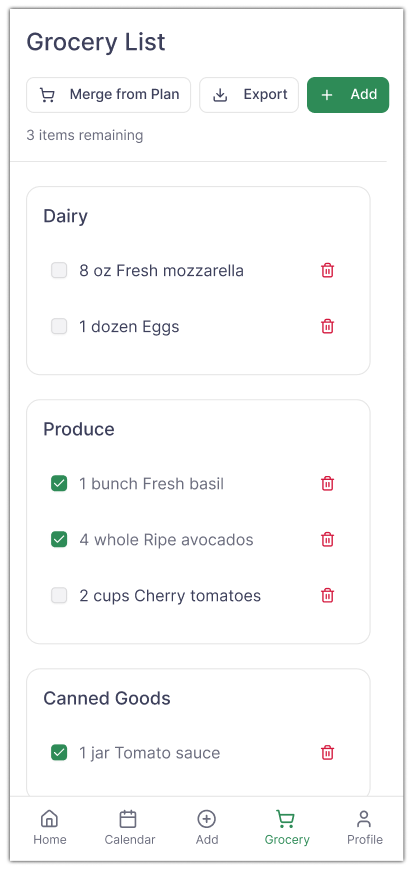
\includegraphics[width=\linewidth]{grocery/list.png}\\[0.15em]
\scriptsize Grocery list
\end{minipage}
\begin{minipage}[!htbp]{0.37\linewidth}\centering
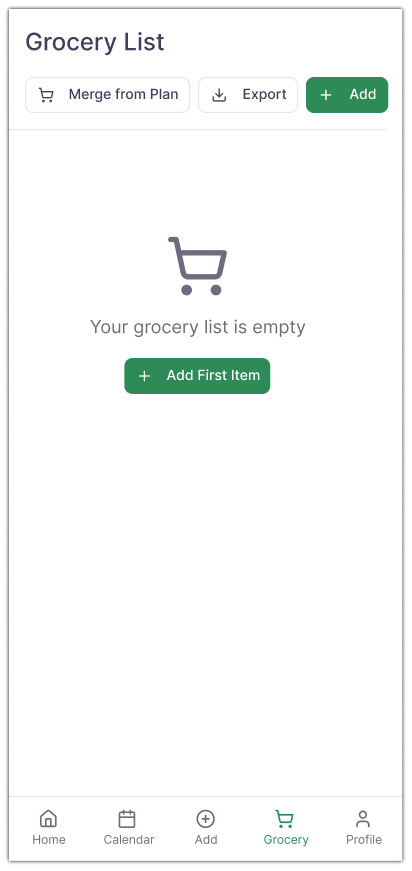
\includegraphics[width=\linewidth]{grocery/empty.png}\\[0.15em]
\scriptsize Empty grocery
\end{minipage}
\caption{Grocery list populated and empty}
\label{fig:grocery-list}
\end{figure}

\textbf{Grocery modals.} These modal menus appear when the add button (top right), and the merge from plan (top left) buttons are clicked. Both menus have clear methods to complete and cancel the action along with an X button in the top corner to easily close the menu.

\begin{figure}[!htbp]
\centering
\begin{minipage}[!htbp]{0.37\linewidth}\centering
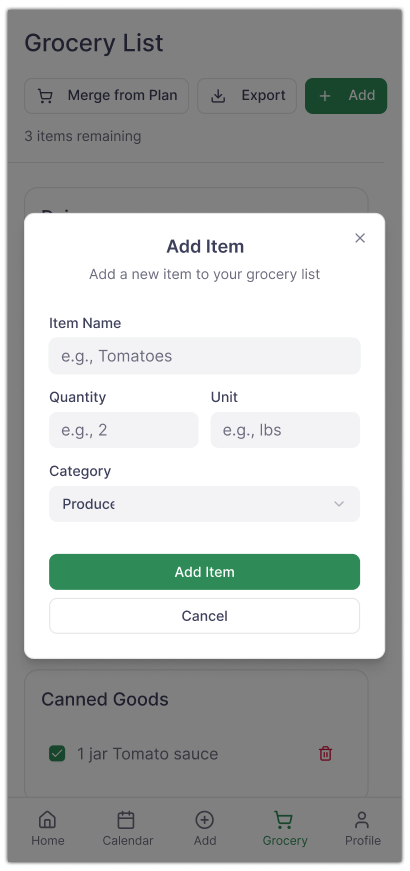
\includegraphics[width=\linewidth]{grocery/add-modal.png}\\[0.15em]
\scriptsize Add grocery item
\end{minipage}
\begin{minipage}[!htbp]{0.37\linewidth}\centering
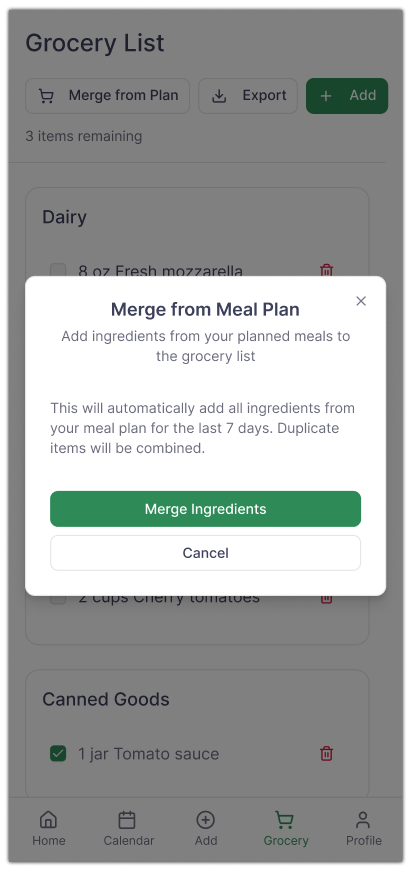
\includegraphics[width=\linewidth]{grocery/merge-modal.png}\\[0.15em]
\scriptsize Merge from plan
\end{minipage}
\caption{Grocery: add-item sheet and merge-from-plan confirmation.}
\label{fig:grocery-modals}
\end{figure}

\newpage
\textbf{Profile and sign-out - } This page contains the user's profile along with their name, bio, goals, and restrictions, all of which are editable from this menu. This page also allows the user to sign out which triggers a modal confirming the action, on confirmation taking them back to the login page (Fig. \ref{fig:auth})

\begin{figure}[!htbp]
\centering
\begin{minipage}[!htbp]{0.32\linewidth}\centering
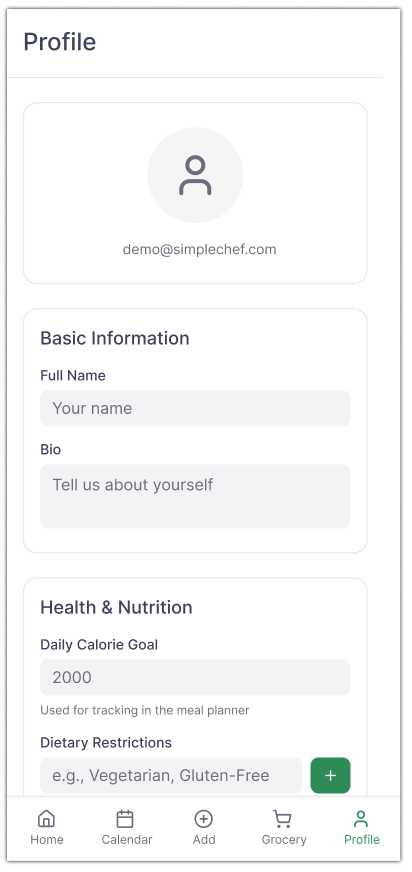
\includegraphics[width=\linewidth]{profile/profile-top.png}\\[0.15em]
\scriptsize Profile (top)
\end{minipage}\hfill
\begin{minipage}[!htbp]{0.32\linewidth}\centering
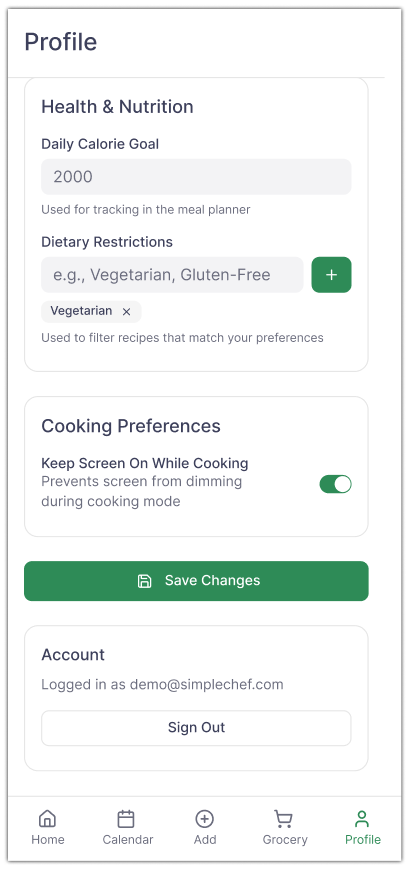
\includegraphics[width=\linewidth]{profile/profile-bottom.png}\\[0.15em]
\scriptsize Profile (bottom)
\end{minipage}\hfill
\begin{minipage}[!htbp]{0.32\linewidth}\centering
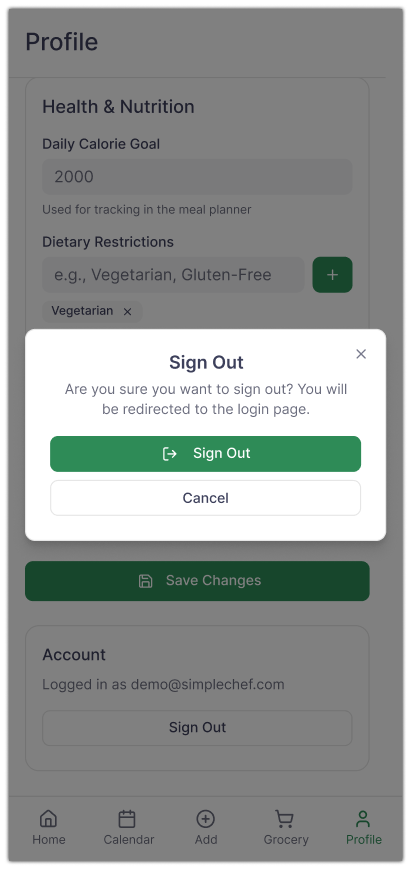
\includegraphics[width=\linewidth]{profile/sign_out-modal.png}\\[0.15em]
\scriptsize Sign out confirmation
\end{minipage}
\caption{Profile: account fields, goals, dietary restrictions, and sign-out confirmation modal.}
\label{fig:profile}
\end{figure}

\subsection{Backend Implementation}

As mentioned earlier the front and backends of the project are completely separated only connecting by a controller that is located in the frontend directory of the project. This allows us to easily expose APIs on the backend of the project for the controller to interacts with and communicate with the presentation layers, making it very easy to iterate on the UI without breaking the business logic.

Below is the shared GitLab repository where the project is currently hosted, it currently contains all the frontend, backend, and documentation of the project so far.

Unfortunately GitLab has a maximum sharing limit of 5 users, so the link cannot be shared for viewing. If the code would like to be viewed you are welcome to ask our group during class, or we can try our best to arrange a time during office hours.

\begin{figure}[H]
\centering
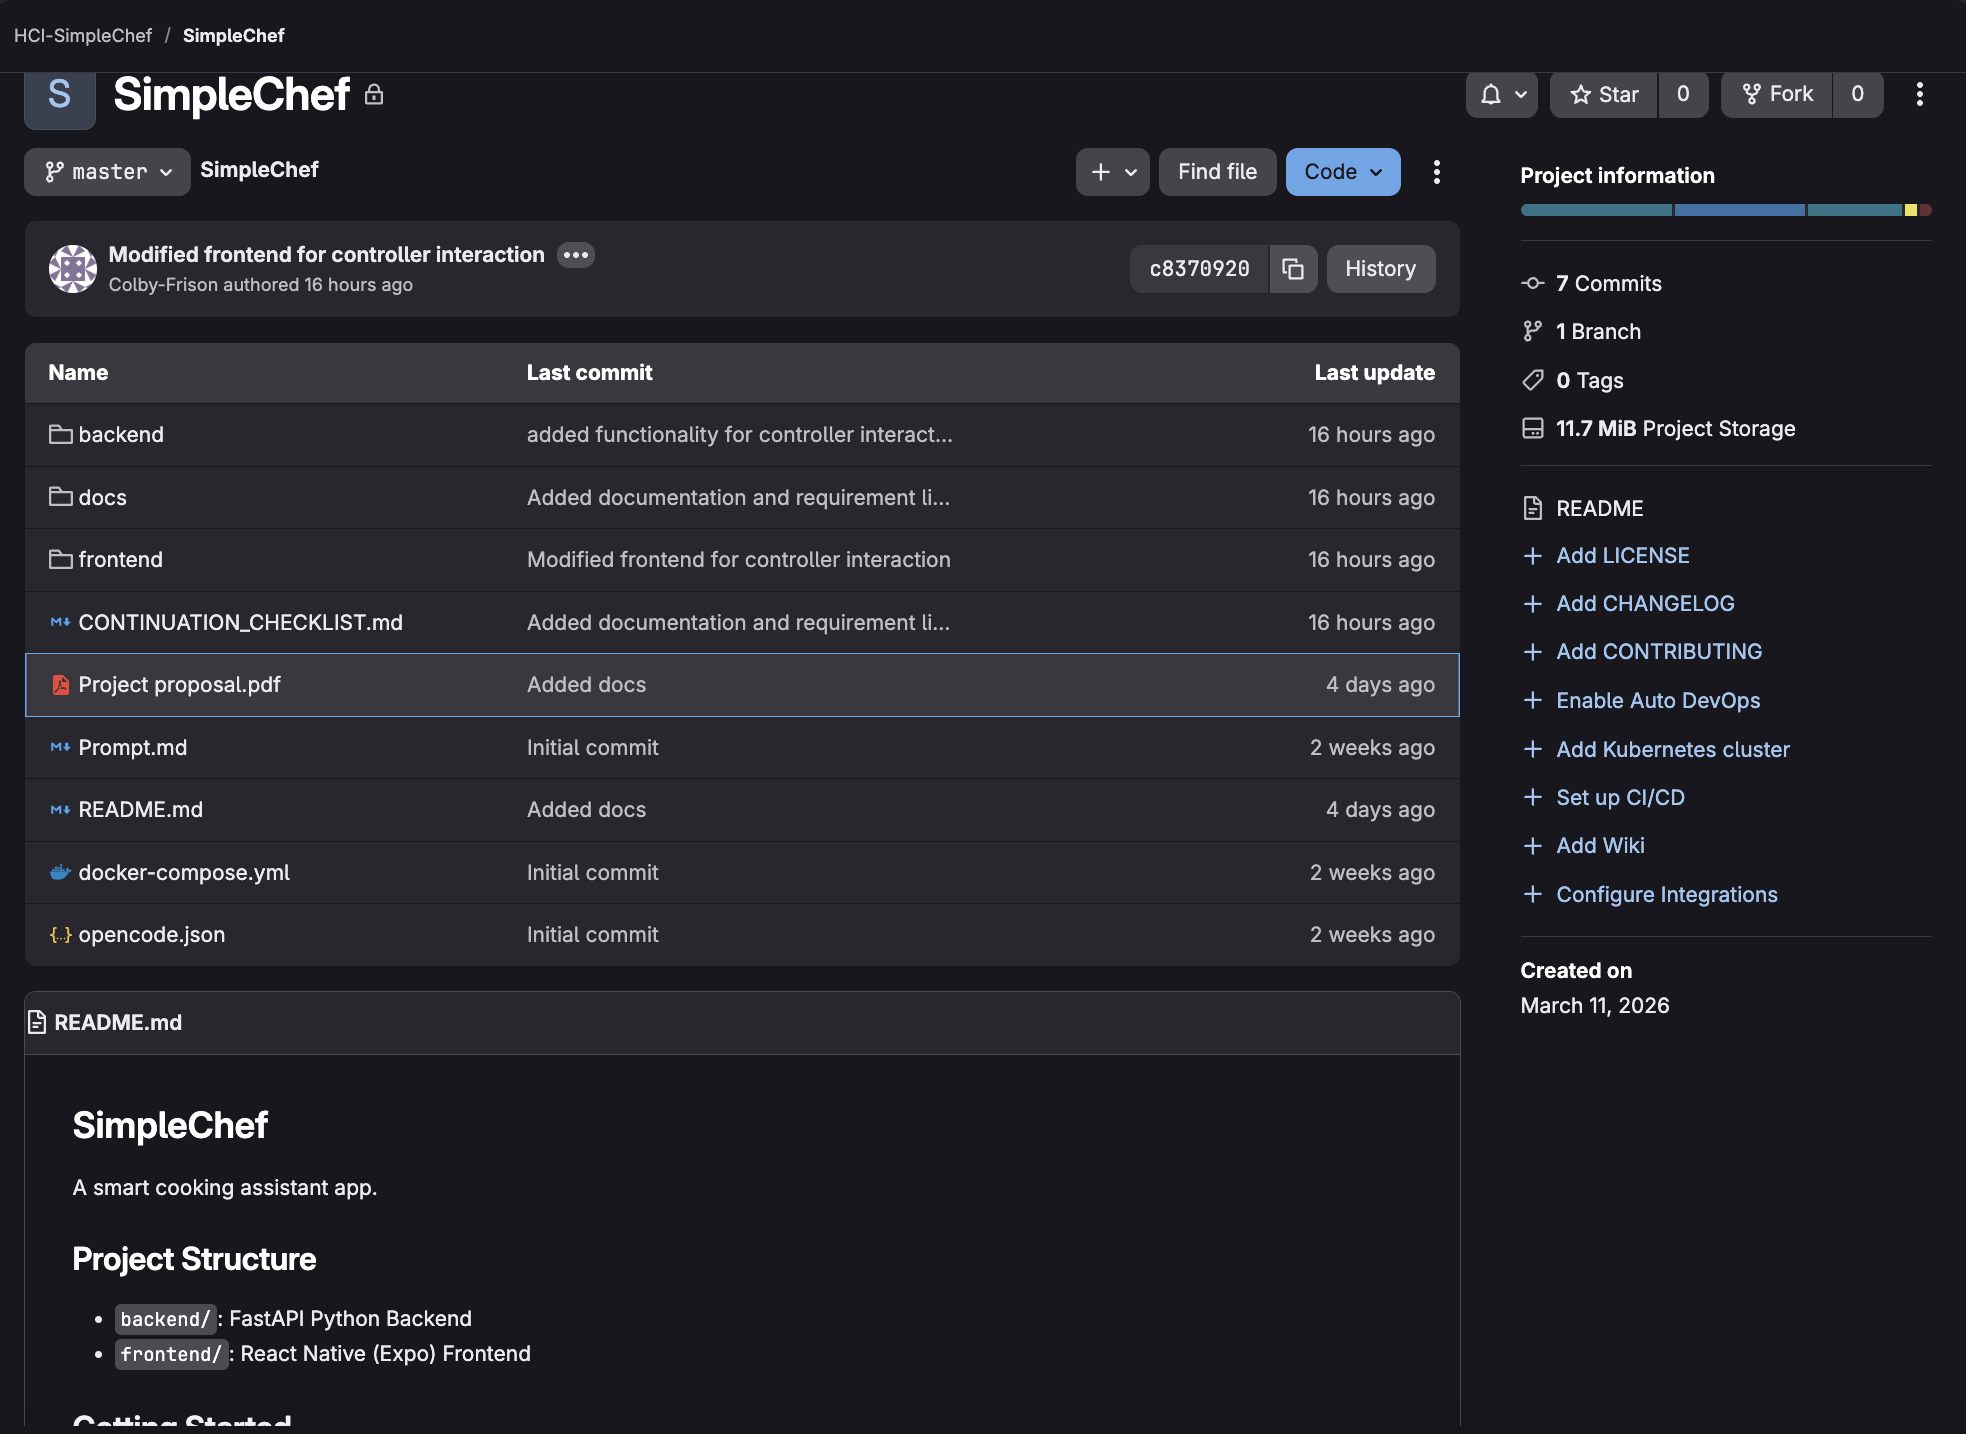
\includegraphics[width=\columnwidth,height=5.5cm,keepaspectratio]{arch/gitlab.png}
\caption{GitLab repository structure and CI setup.}
\label{fig:gitlabd-2}
\end{figure}

The following images are a very quick mockup for a frontend to demonstrate backend functionality. All of these images directly correspond to images shown above, but clearly low-fidelity. Not all pages are shown because this low-fidelity mockup for functionality doesn't have all pages, just the ones that show core functionality, but we assure all the backend endpoints are present.
The bottom bar still remains present through all pages, but contains an extra "explore" tab which is just a diagnostic tool for Expo Go (used for testing the project), this is not an actual element in the front or backend it is simply an artifact of the testing environment.


\begin{figure}[H]
\centering
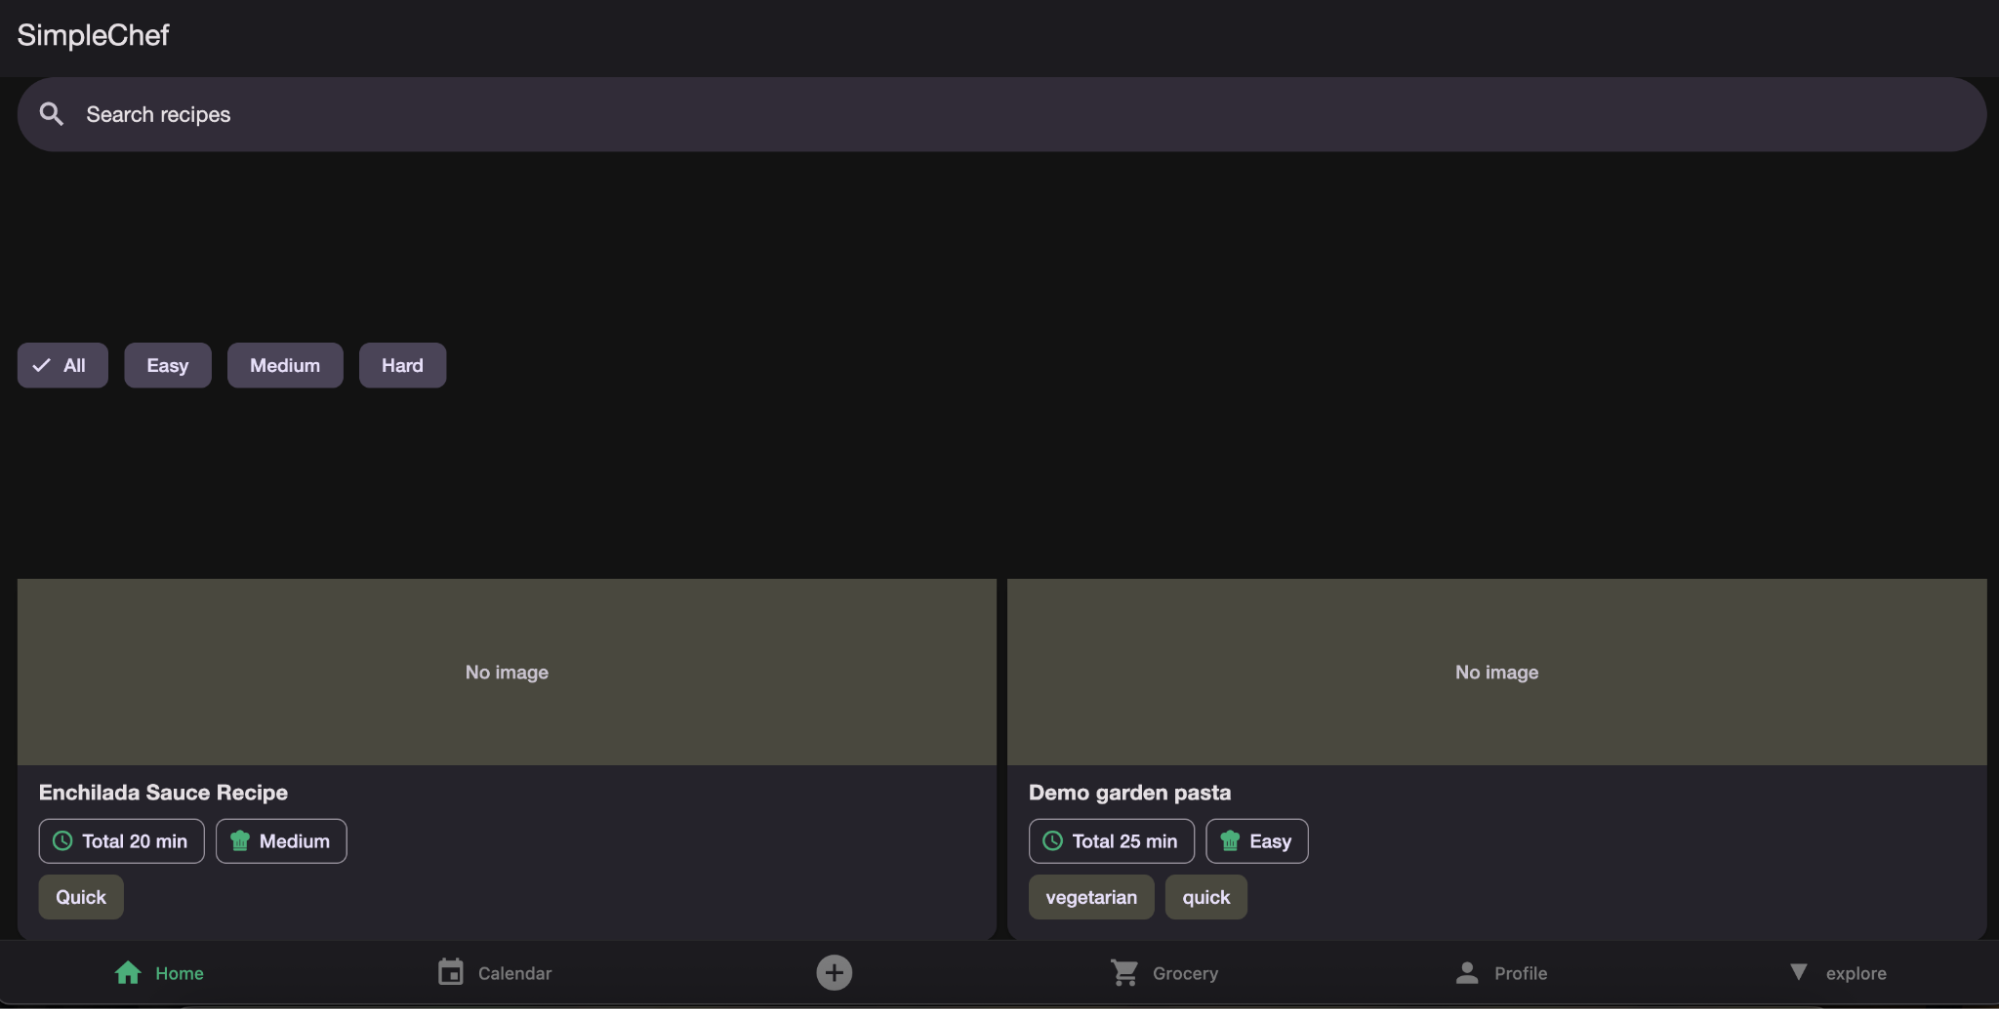
\includegraphics[width=\columnwidth,height=4.5cm,keepaspectratio]{screenshots/home-real.png}
\vspace{-.3cm}
\caption{Home page with search, model filter categories, and some example recipes.}
\label{fig:backend-home}
\end{figure}
\vspace{-.2cm}
\begin{figure}[H]
\centering
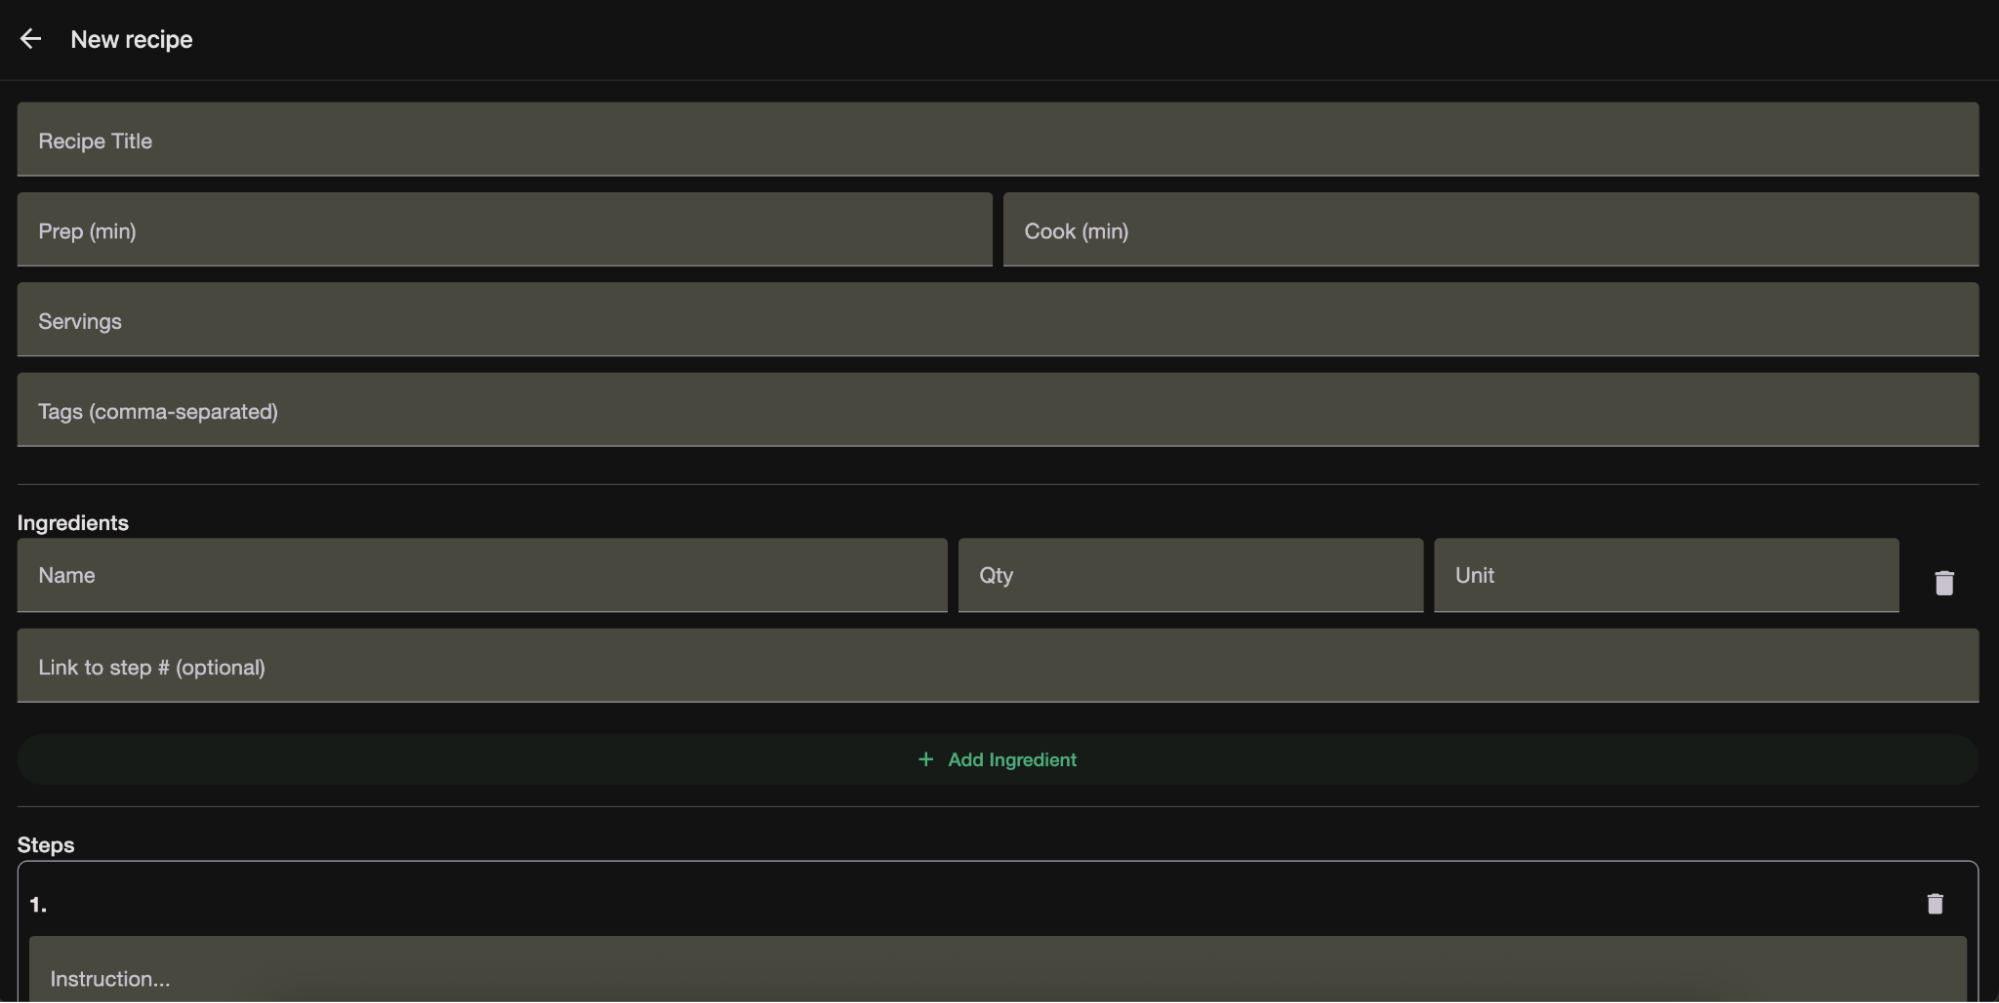
\includegraphics[width=\columnwidth,height=4.5cm,keepaspectratio]{screenshots/create-recipe-real.png}
\vspace{-.3cm}
\caption{Manual recipe input page with templates for recipe info, ingredients and steps. A back button is present to go to the previous page.}
\label{fig:Backend-recipe}
\end{figure}
\vspace{-.2cm}
\begin{figure}[H]
\centering
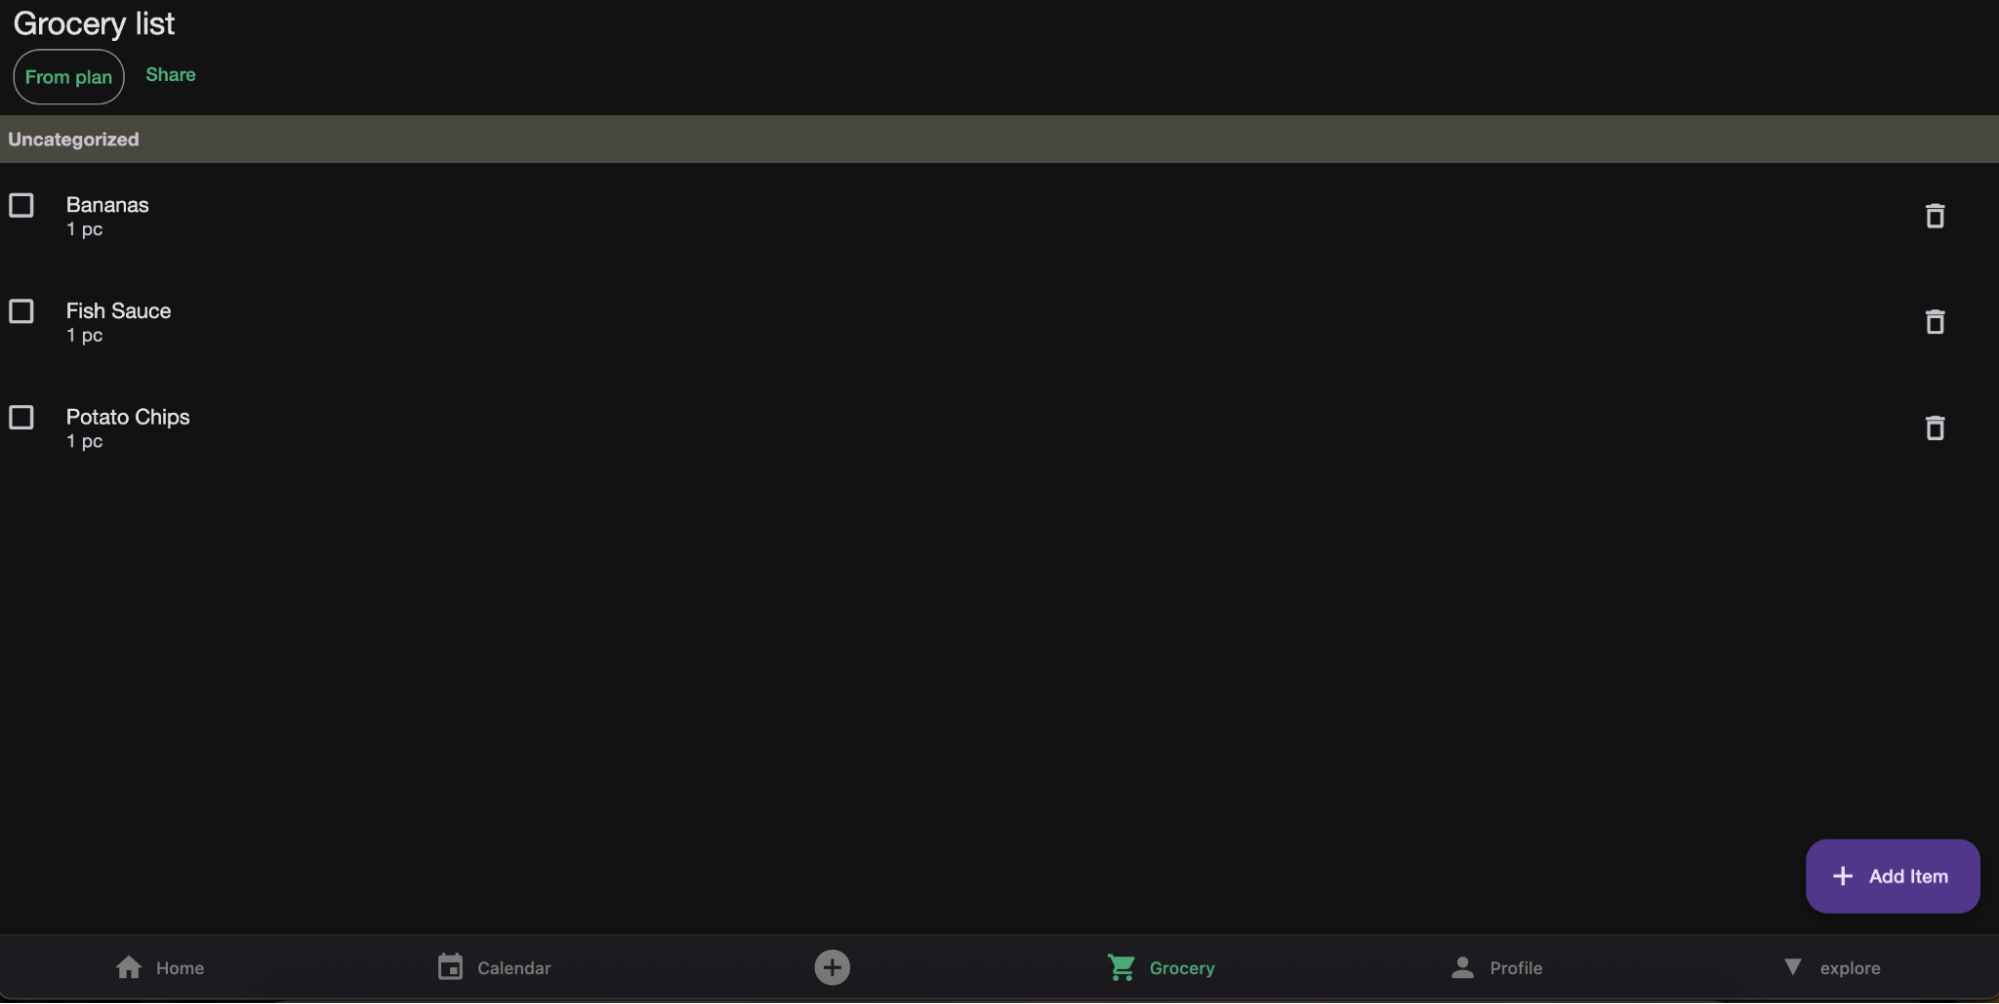
\includegraphics[width=\columnwidth,height=4.5cm,keepaspectratio]{screenshots/grocery-real.png}
\vspace{-.3cm}
\caption{Grocery list with example items. From plan, share and add items are present for list sharing and modification.}
\label{fig:backend grocery list}
\end{figure}

\begin{figure}[H]
\centering
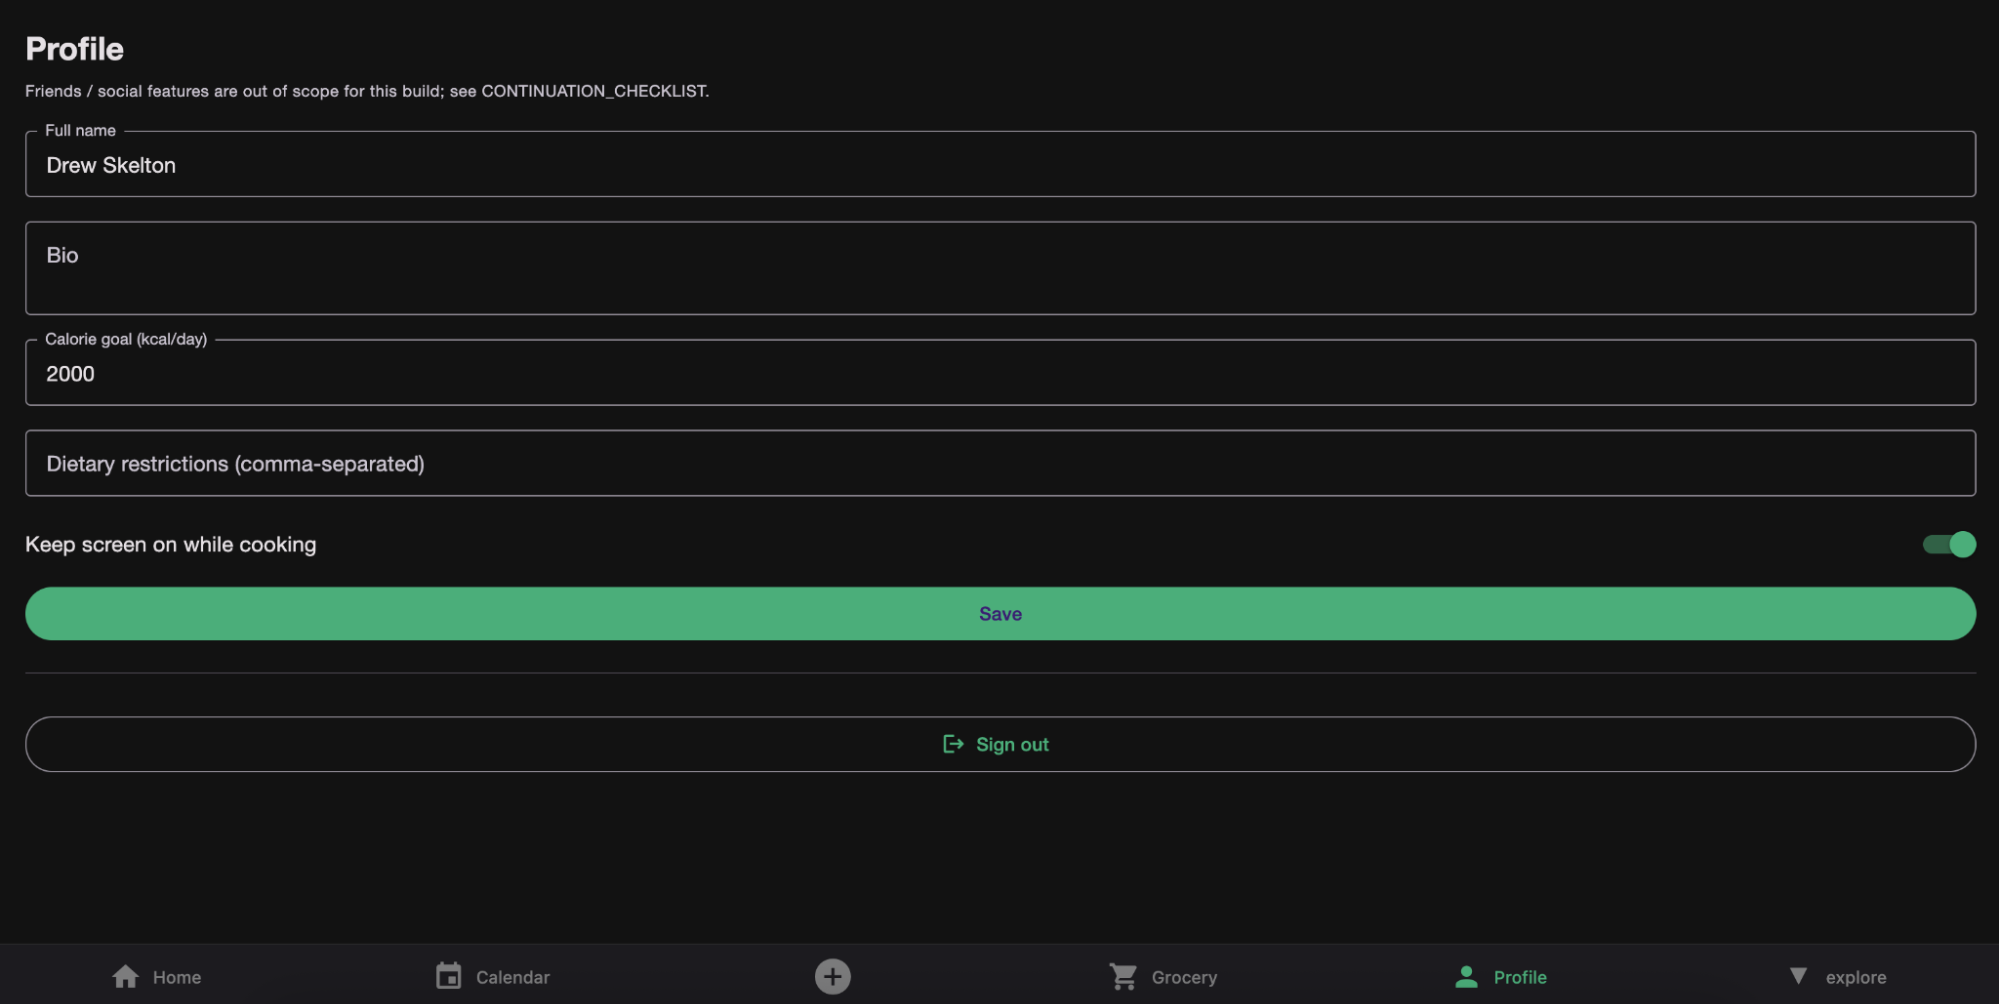
\includegraphics[width=\columnwidth,height=4.5cm,keepaspectratio]{screenshots/profile-real.png}
\caption{GitLab repository structure and CI setup.}
\label{fig:gitlab}
\end{figure}

\section{Future Work and To-Do}
Remaining work is organized by similarity. The following tables detail this remaining work
\vspace{-.2cm}
\begin{table}[!htbp]
\centering
\caption{Near-term tasks (late March--April).}
\label{tab:near}
\begin{tabular}{|@{}>{\raggedright\arraybackslash}p{0.28\linewidth}|>{\raggedright\arraybackslash}p{0.62\linewidth}@{}|}
\hline
\textbf{Task} & \textbf{Notes} \\
\hline
Expose Home time/tag filters in UI & API ready; align with profile dietary defaults. \\\hline
Month calendar indicators + statistics & Dots/trends per proposal; optional charts. \\\hline
Replace mock AI parser & Keep verify-and-edit UX; improve extraction and errors. \\\hline
Figma high-fi + navigation delta & Cooking chrome vs.\ tabs; see Figma requirements doc. \\
\hline
\end{tabular}
\end{table}

\begin{table}[!htbp]
\centering
\caption{Mid-term tasks (proposal Weeks~5--7 and polish).}
\label{tab:mid}
\begin{tabular}{|@{}>{\raggedright\arraybackslash}p{0.28\linewidth}|>{\raggedright\arraybackslash}p{0.62\linewidth}@{}|}
\hline
\textbf{Task} & \textbf{Notes} \\
\hline
Image / video import & OCR or model pipeline; loading and failure states. \\\hline
Grocery inline edit + reorder & Persisted ordering if required by product. \\\hline
Optional statistics & Trends vs.\ goals using meal logs. \\\hline
Friends / sharing & If in scope: APIs and UI. \\\hline
\end{tabular}
\end{table}

\begin{table}[!htbp]
\centering
\caption{Course deliverables tied to evaluation and documentation.}
\label{tab:course}
\begin{tabular}{|@{}>{\raggedright\arraybackslash}p{0.28\linewidth}|>{\raggedright\arraybackslash}p{0.62\linewidth}@{}|}
\hline
\textbf{Task} & \textbf{Notes} \\
\hline
Usability testing & Task scripts: browse, cook with timers, plan, grocery. \\\hline
Heuristic and accessibility pass & Contrast, touch targets, legibility while cooking~\cite{wcag21}. \\\hline
Final demo and report & Live demo, design rationale, user analysis per syllabus. \\\hline
\end{tabular}
\end{table}

\section{Project Plan and Concept}
All the previous section primarily go over what we are using or what we have, this section will go over the plan for the project, and some of the system's architecture. This will include the user flow front/backend architecture and the database diagram.

% User flow: top-down entry spine, then five tab columns spread across the page.
% Column x-positions (cm): Add=-9, Home=-4.5, Calendar=0, Grocery=4.5, Profile=9
% Rows (y, negative = down): entry=0, auth=-1.4, home=-3.2, tab-root=-5.0, sub1=-6.8, sub2=-8.4, sub3=-10.0
\begin{figure*}[!htbp]
\centering
\resizebox{\textwidth}{!}{%
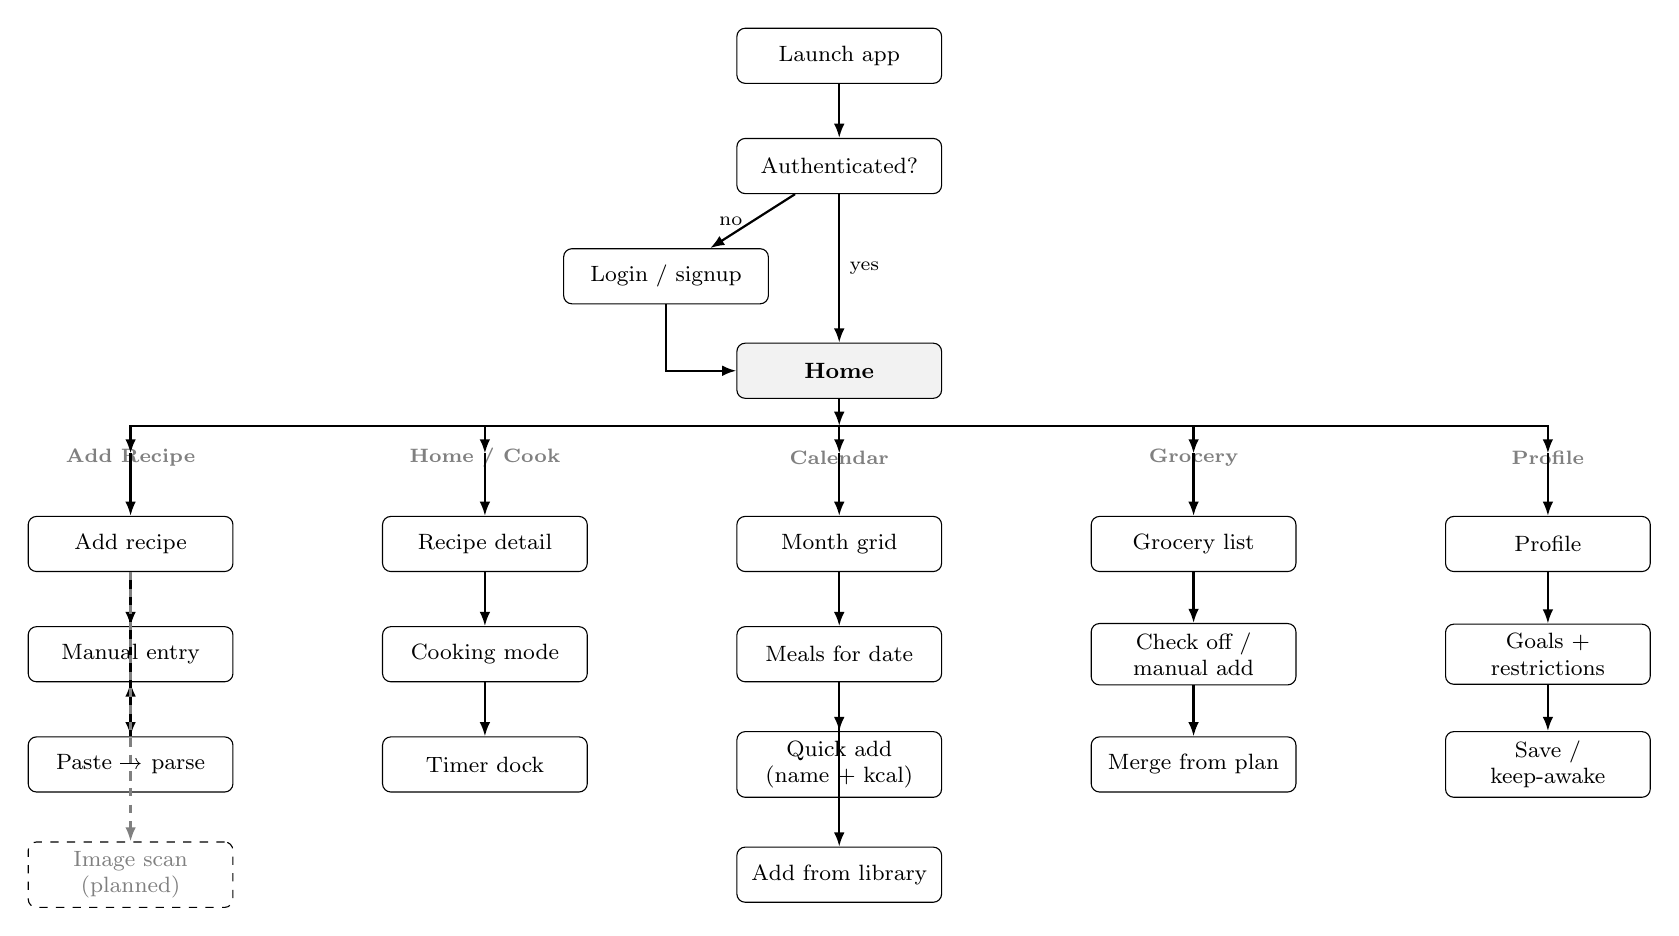
\begin{tikzpicture}[
  font=\footnotesize,
  % Standard implemented node
  box/.style={rectangle, draw, rounded corners=3pt,
              minimum width=2.6cm, minimum height=0.7cm, align=center,
              fill=white},
  % Planned / future node
  plan/.style={rectangle, draw, dashed, rounded corners=3pt,
               minimum width=2.6cm, minimum height=0.7cm, align=center,
               fill=white, text=gray},
  % Thin column-header label (no box)
  hdr/.style={font=\scriptsize\bfseries, text=gray},
  arr/.style={-{Latex[length=1.8mm]}, thick},
  darr/.style={-{Latex[length=1.8mm]}, thick, dashed, gray}
]

% ── Entry spine (centred) ──────────────────────────────────────────────────
\node[box]                      (launch) at (0, 0)    {Launch app};
\node[box]                      (auth)   at (0,-1.4)  {Authenticated?};
\node[box]                      (login)  at (-2.2,-2.8) {Login / signup};
\node[box, fill=gray!10, font=\footnotesize\bfseries]
                                (home)   at (0,-4.0)  {Home};

\draw[arr] (launch) -- (auth);
\draw[arr] (auth)   -- node[left,  font=\scriptsize] {no}  (login);
\draw[arr] (auth)   -- node[right, font=\scriptsize] {yes} (home);
\draw[arr] (login)  |- (home);   % login re-joins home spine

% ── Column header labels ───────────────────────────────────────────────────
\node[hdr] at (-9,   -5.1) {Add Recipe};
\node[hdr] at (-4.5, -5.1) {Home / Cook};
\node[hdr] at ( 0,   -5.1) {Calendar};
\node[hdr] at ( 4.5, -5.1) {Grocery};
\node[hdr] at ( 9,   -5.1) {Profile};

% Horizontal bus line from Home to each column root
\draw[arr] (home) -- ++(0,-0.7) coordinate (bus);
\draw[arr] (bus) -- ++(-9,0)   -- ++(0,-0.35) coordinate (addtop);
\draw[arr] (bus) -- ++(-4.5,0) -- ++(0,-0.35) coordinate (htop);
\draw[arr] (bus) -- ++(0,0)    -- ++(0,-0.35) coordinate (caltop);
\draw[arr] (bus) -- ++(4.5,0)  -- ++(0,-0.35) coordinate (groctop);
\draw[arr] (bus) -- ++(9,0)    -- ++(0,-0.35) coordinate (proftop);

% ── Add Recipe column ──────────────────────────────────────────────────────
\node[box]  (add)    at (-9,-6.2)  {Add recipe};
\node[box]  (manual) at (-9,-7.6)  {Manual entry};
\node[box]  (parse)  at (-9,-9.0)  {Paste → parse};
\node[plan] (img)    at (-9,-10.4) {Image scan\\(planned)};

\draw[arr]  (addtop) -- (add);
\draw[arr]  (add)    -- (manual);
\draw[arr]  (add)    -- (parse);
\draw[arr]  (parse)  -- (manual);   % parse verifies via manual screen
\draw[darr] (add) to[out=270,in=90] (img);

% ── Home / Cook column ────────────────────────────────────────────────────
\node[box] (detail) at (-4.5,-6.2) {Recipe detail};
\node[box] (cook)   at (-4.5,-7.6) {Cooking mode};
\node[box] (dock)   at (-4.5,-9.0) {Timer dock};

\draw[arr] (htop)   -- (detail);
\draw[arr] (detail) -- (cook);
\draw[arr] (cook)   -- (dock);

% ── Calendar column ───────────────────────────────────────────────────────
\node[box] (cal)   at (0,-6.2)  {Month grid};
\node[box] (meals) at (0,-7.6)  {Meals for date};
\node[box] (qadd)  at (0,-9.0)  {Quick add\\(name + kcal)};
\node[box] (lib)   at (0,-10.4) {Add from library};

\draw[arr] (caltop) -- (cal);
\draw[arr] (cal)    -- (meals);
\draw[arr] (meals)  -- (qadd);
\draw[arr] (meals)  to[out=270,in=90] (lib);

% ── Grocery column ────────────────────────────────────────────────────────
\node[box] (groc) at (4.5,-6.2) {Grocery list};
\node[box] (gchk) at (4.5,-7.6) {Check off /\\manual add};
\node[box] (gsync)at (4.5,-9.0) {Merge from plan};

\draw[arr] (groctop) -- (groc);
\draw[arr] (groc)    -- (gchk);
\draw[arr] (gchk)    -- (gsync);

% ── Profile column ────────────────────────────────────────────────────────
\node[box] (prof)  at (9,-6.2) {Profile};
\node[box] (goals) at (9,-7.6) {Goals +\\restrictions};
\node[box] (save)  at (9,-9.0) {Save /\\keep-awake};

\draw[arr] (proftop) -- (prof);
\draw[arr] (prof)    -- (goals);
\draw[arr] (goals)   -- (save);

\end{tikzpicture}%
}
\caption{User flow: entry spine fans into five tab columns. Solid arrows =
implemented; dashed gray = planned.}
\label{fig:flow}
\end{figure*}
The figure above contains the flowchart for the user, detailing how the user with experience the system. This is also a general list of features of the project and where they are located. It is likely this chart will change or grow as current features are finalized, or extended features are implemented.

The figure below shows the high level implementation of the project, the back end connecting to the frontend through FastAPI with the API call to the AI being launched from the controller. as this feature progresses the AI may be handled in the backend entirely, but that will be discussed when decide to move forward with implementing this feature.
\begin{figure}[!htbp]
\centering
\resizebox{\columnwidth}{!}{%
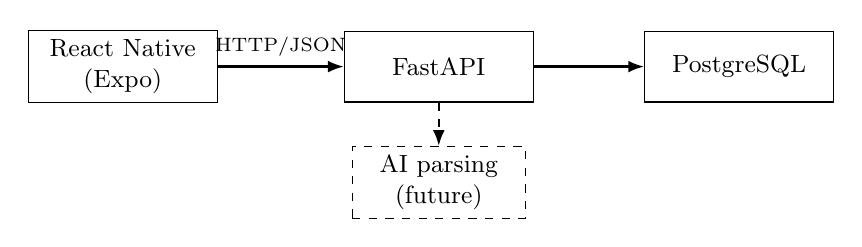
\begin{tikzpicture}[
  font=\small,
  srv/.style={rectangle, draw, minimum width=2.4cm, minimum height=0.9cm, align=center},
  future/.style={rectangle, draw, dashed, minimum width=2.2cm, minimum height=0.75cm, align=center},
  arr/.style={-{Latex[length=2mm]}, thick}
]
  \node[srv] (rn) {React Native\\(Expo)};
  \node[srv, right=1.6cm of rn] (api) {FastAPI};
  \node[srv, right=1.4cm of api] (db) {PostgreSQL};
  \node[future, below=0.55cm of api] (ai) {AI parsing\\(future)};
  \draw[arr] (rn) -- node[above, font=\scriptsize] {HTTP/JSON} (api);
  \draw[arr] (api) -- (db);
  \draw[arr, dashed] (api) -- (ai);
\end{tikzpicture}%
}
\vspace{-.3cm}
\caption{System context: mobile client, API layer, database; optional AI service for parsing.}
\label{fig:arch}
\end{figure}

The following image is the ER diagram (Entity relationship diagram) of our Postgre-SQL database. We are currently hosting the database in a docker image that is run while testing, but when the project is deployed we will have to find an alternative host. Due to the small scale of data likely going into the database we have not worried much about its efficiency, but prior to deployment we will likely refactor and stress test the DB to ensure its stability.
\begin{figure}
    \centering
    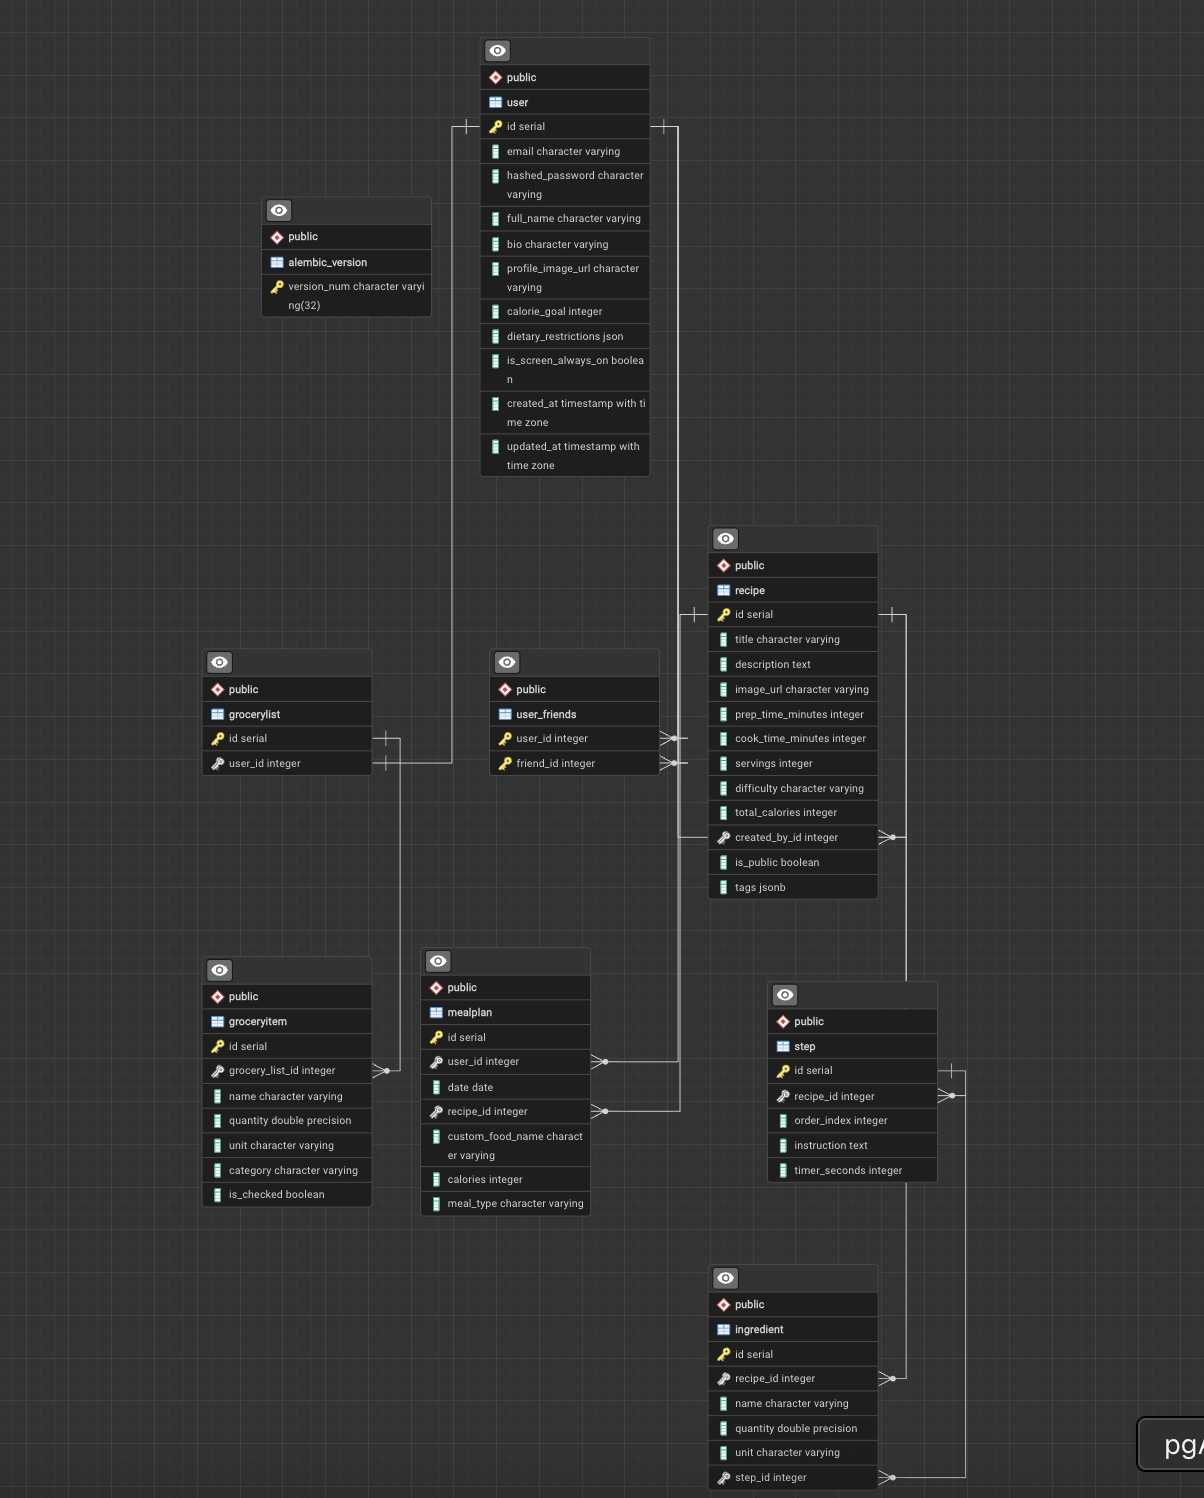
\includegraphics[width=.7\linewidth]{figures/arch/er-diagram.png}
    \caption{PostgreSQL entity-relationship diagram showing all current models
and their associations.}
    \label{fig:ER-diagram}
\end{figure}

\newpage
\section{Project Progress Timeline}
The following table~\ref{tab:gantt} is a simple overview of specific task completion, and tasks still needed to be done all the way to the final presentation. Dates are present for a soft due date for group members, and small notes are included for added detail.

%Overleaf doesn't like \addlinespace
\begin{table*}[!htbp]
\centering
\caption{Milestone summary (Spring 2026, indicative dates).}
\label{tab:gantt}
\begin{tabular}{|@{}>{\raggedright\arraybackslash}p{0.34\linewidth}|>{\raggedright\arraybackslash}p{0.12\linewidth}|>{\raggedright\arraybackslash}p{0.18\linewidth}|>{\raggedright\arraybackslash}p{0.28\linewidth}@{}|}
\hline
\textbf{Phase/task} & \textbf{Status} & \textbf{Span (approx.)} & \textbf{Notes} \\
\hline
Proposal and wireframe & Done & Feb 1--14 & Scope and specs \\
Repository docs (Figma req., traceability, arch.) & Done & Mar 20--28 & Single sources under \texttt{docs/} \\
Frontend controller layer & Done & Mar 20--28 & \texttt{frontend/controllers/} \\
Backend API and database & Done & Feb 15--Mar 7 & Models, migrations, routers \\
Auth and profile & Done & Feb 20--Mar 28 & JWT, \texttt{/users/me}, PATCH profile \\
Recipe library and detail & Done & Feb 25--Mar 10 & List, detail, filters (API) \\
Cooking mode and timer dock & Done & Mar 1--Mar 14 & Steps, mise, timers \\
Add recipe (manual + parse) & Done & Mar 5--Mar 15 & Verify-and-edit path \\
Meal plan API and calendar UI & Done & Mar 8--Mar 28 & Grid, library add, day summary \\
Grocery list + merge from plan & Done & Mar 10--Mar 28 & Sections, merge, share \\
\hline
\addlinespace
\hline
Figma high-fi + filter UI parity & Active & Mar 22--Apr 10 & Match \texttt{FIGMA\_UI\_...} \\
Real AI text parsing & Planned & Mar 25--Apr 8 & Replace mock service \\
Month indicators + statistics UI & Planned & Apr 1--Apr 20 & Proposal polish \\
\hline
\addlinespace
\hline
Usability tests on build & Planned & Apr 5--Apr 15 & Scripted tasks \\
Heuristics and accessibility & Planned & Apr 12--Apr 20 & WCAG-oriented fixes~\cite{wcag21} \\
Final demo preparation & Planned & Apr 18--Apr 28 & Presentation and polish \\
Final documentation deadline & Milestone & May 3 & Final report (syllabus) \\
\hline
\end{tabular}
\end{table*}

\begin{figure*}
    \centering
    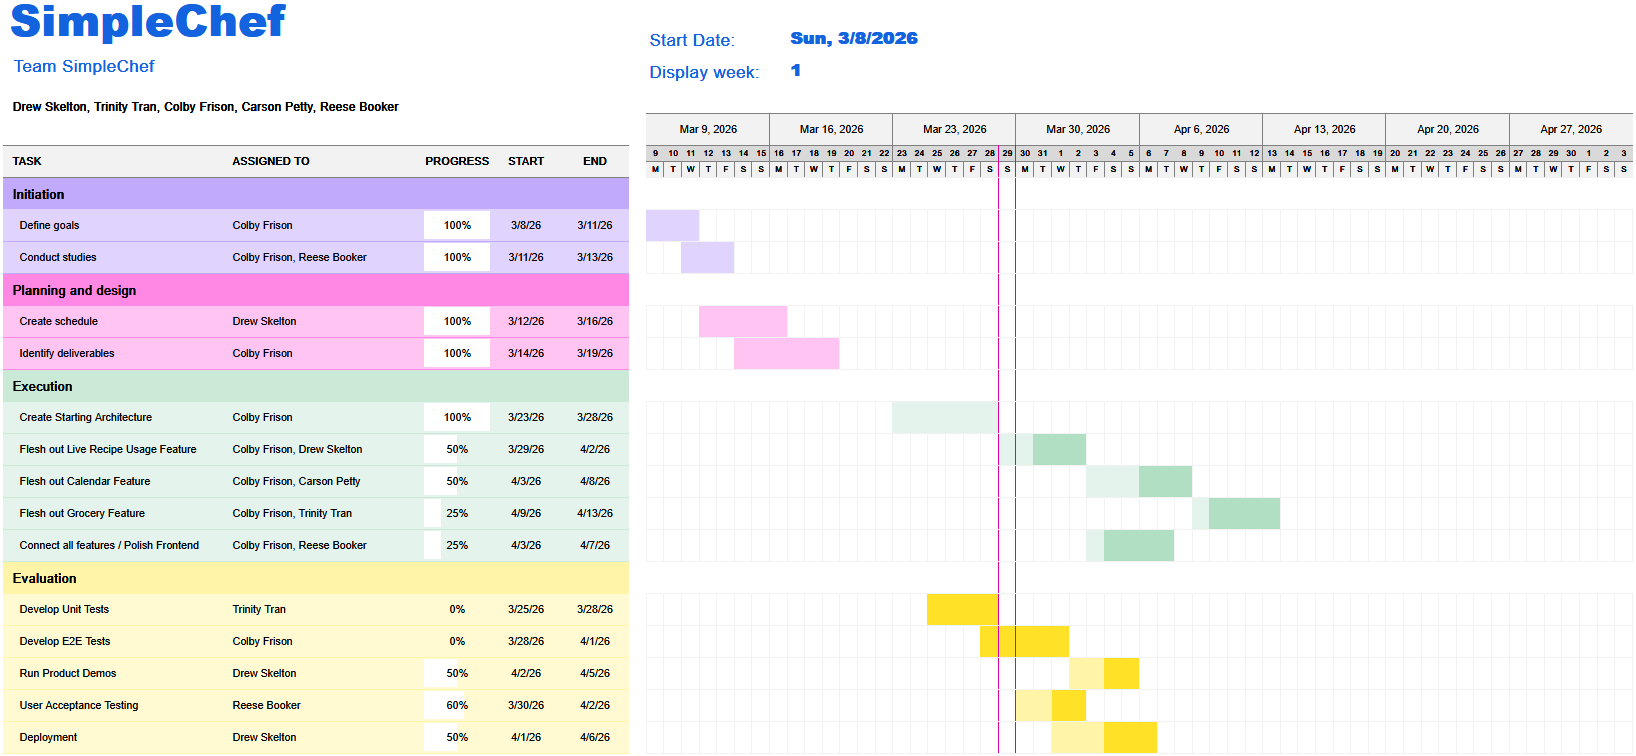
\includegraphics[width=1\linewidth]{figures/screenshots/Gantt-chart.png}
    \vspace{-.3cm}
    \caption{High-fidelity Gantt chart of project plan with member assignments}
    \label{fig:placeholder}
\end{figure*}
The image above is a higher fidelity Gantt chart that includes member participation, and generally a more recognizable format for project organization. This chart only goes up to April 13th, as the presentations start on the 9th so we would like to have a majority of the project done by then.

\subsection{Potential Issues}
\paragraph{Parser}
The manual entry for the recipe is very consistent and yields good results for recipes, but can be time-consuming and tedious if it is needed to be done for many recipes to transfer a user's recipe library. For this reason the parser of very important in gaining and retaining users, and ensuring a good experience and good HCI. Hence, the parser needs to be quite good, or we need to have another method to importing recipes. Also with an approach of using AI, we would have to optimize token usage to not be super expensive, additionally if an external API is used we have to moderate it to ensure it still functions after updates or changes. 

\paragraph{Project Deadline}
There is still a sizable amount of work to do before we can "ship the product", and the project presentations start far before the final deliverable, so ensuring the project is in a presentable state by then presentation may require some clever design. Additionally, we have many features that we deem to be "extended features" meaning they are not crucial to the function of the system, but their implementation would improve the user experience and the overall HCI. These features may have to be abandoned if the crucial features cannot be polished quickly.

\paragraph{Usability across users types}
This project has been entirely designed and critiqued by computer science students/professors. And it is likely that the people testing it will also be familiar with technology, so ensuring the product is usable by novice, intermediate, and expert users (in the realm of technology) may be difficult.

\section{Conclusion}
SimpleChef has moved from a simple design specification and requirement list to a functional prototype with a documented separation between presentation (Expo routes and components) and application logic (controller hooks), backed by a traceable API and SRS mapping. The figures in Section\textbf{~\ref{sec:evidence}} document the intended high-fidelity UI, although these designs are not yet connected to the API, backend support and controller wiring provide a direct path to integrate this high fidelity design. Some of the requirements implemented so far include the ability for the user to browse and filter manually entered recipes, inspect detail, run step-by-step cooking with a timer dock, add recipes manually or via parse-then-edit, plan meals on a monthly calendar with day-level calorie summaries, merge groceries from plans, and edit profile settings. Tasks that still need to be completed that were mentioned in the initial project proposal include: richer Home filters in the UI, calendar visual density and statistics, recipe parsing, grocery inline editing and reorder, optional social features (for easily sharing recipes), and evaluation activities (usability testing, heuristic review, accessibility).

\bibliographystyle{IEEEtran}
\bibliography{references}

\newpage
\section*{Figure and Table Index}
\noindent\textit{In the PDF, each line below links to the corresponding figure or table (click the text or page number).}

\begingroup
\footnotesize
\setlength{\parskip}{0.35em}
\renewcommand{\listfigurename}{\normalsize\normalfont\bfseries Figures}
\renewcommand{\listtablename}{\normalsize\normalfont\bfseries Tables}
\listoffigures
\vspace{1.25em}
\listoftables
\endgroup

\end{document}
